\newpage\null\par
\section{实验二\hspace{1em}大气环境质量现状评价}
\subsection{教学目的与要求}
\noindent\textbf{教学目的:}通过某城市生活垃圾环保发电厂为实例来进行大气环境质量评价。\newline
\noindent\textbf{教学要求:}
\begin{enumerate}
    \item 熟悉大气环境预测软件AERSCREEN在大气环境质量预测与评价中的应用,掌握EIAProA2018软件模型估算最大落地浓度和$\mathrm{D_{10\%}}$确定评价工作等级的基本方法。
    \item 利用EIAProA2018软件估算最大落地浓度和$\mathrm{D_{10\%}}$确定评价工作等级和范围,并附上软件主要操作步骤。
    \item 制定某城市生活垃圾环保发电厂的大气环境质量现状监测方案(包含范围、布点(按要求给出布点图)、因子、方法、时期、次数等)。
\end{enumerate}

\subsection{实验报告背景}
\begin{enumerate}
    \item 确定某城市生活垃圾环保发电厂大气环境质量评价工作等级与评价范围
    
    根据项目初步分析,选择 $1\sim3$ 种主要污染物,分别计算每一种污染物的最大地面浓度占标率 $P_i$(第 $i$ 个污染物),及第 $i$ 个污染物的地面浓度达标准限值10\%时所对应的最远距离$\mathrm{D_{10\%}}$。
    \begin{equation} \label{eq:The maximum ground concentration of the pollutant is standardized}
        P_i=\dfrac{C_i}{C_{0i}}\times 100\%
    \end{equation}
    式中:$P_i$——第i个污染物的最大地面空气质量浓度占标率,\%;
    \newline\phantom{式中:}$C_i$——采用估算模型计算出的第$i$个污染物的最大1 h地面空气质量浓度,μg/m$^3$;
    \newline\phantom{式中:}$C_{oi}$——第$i$个污染物的环境空气质量浓度标准,μg/m$^3$。一般选用GB 3095中1h平均质量浓度的二级浓度限值,如项目位于一类环境空气功能区,应选择相应的一级浓度限值;对该标准中未包含的污染物,使用评价标准\cite{HJ2.2-2018}确定的各评价因子1 h平均质量浓度限值。对仅有8h平均质量浓度限值、日平均质量浓度限值或年平均质量浓度限值的,可分别按2倍、3倍、6倍折算为1 h平均质量浓度限值。

    \begin{table}[H]
        \centering
        \caption{评价等级判别表\cite{HJ2.2-2018}}
        \begin{tabular}{cc}
        \toprule
        评价工作等级 & 评价工作分级判据 \\
        \midrule
        一级评价 & $P_{\text{max}} \geqslant  10\%$ \\
        二级评价 & $1\% \leqslant  P_{\text{max}} < 10\%$ \\
        三级评价 & $P_{\text{max}} < 1\%$ \\
        \bottomrule
        \end{tabular}
    \end{table}

    \item 污染源及项目周边条件基本信息
    
    \begin{table}[H]
        \centering
        \caption{污染源及项目周边条件基本信息}
        \begin{tabular}{p{0.3\textwidth}p{0.15\textwidth}p{0.1\textwidth}}
            \toprule
            名称 & 值 & 单位 \\
            \midrule
            污染源总量排放速率 & 60000 & Nm$^3$/h \\
            烟囱高度 & 130 & m \\
            烟囱内径 & 5 & m \\
            排放口温度 & 293 & K \\
            烟气出口速度 & 15 & m/s \\
            所在区域最低气温 & $-6$ & ℃ \\
            所在区域最高气温 & 44 & ℃ \\
            \midrule
            地点 & 农村地区 & - \\
            区域湿度条件 & 潮湿 & - \\
            \bottomrule
        \end{tabular}
        \label{tab:Basic information on pollution sources and surrounding conditions of the project}
    \end{table}

    \item 污染物标准
    
    计算污染物的源强(烟气流量与污染物浓度相乘),利用EIAProA2018软件估算出每个污染物的最大出落地浓度,再与环境空气质量标准(二级小时浓度)相比计算$P_i$。
    \begin{table}[H]
        \centering
        \caption{污染物排放值}
        \resizebox{\textwidth}{!}{
        \begin{tabular}{cccccc}
        \toprule
        序号    & 污染物名称 & 单位    & 工业企业设计卫生标准 & 项目排放值 & 污染源强(kg/h) \\
        \midrule
        1     & 颗粒物   & μg/Nm$^3$ & 900   & 50    & 0.003 \\
        2     & HCl   & μg/Nm$^3$ & 50    & 50    & 0.003 \\
        3     & HF    & μg/Nm$^3$ & 20    & 2     & 0.00012 \\
        4     & $\mathrm{SO_x}$   & μg/Nm$^3$ & 500   & 250   & 0.015 \\
        5     & $\mathrm{NO_x}$   & μg/Nm$^3$ & 250   & 150   & 0.009 \\
        6     & CO    & μg/Nm$^3$ & 10000 & 100   & 0.006 \\
        \bottomrule
        \end{tabular}}
        \label{tab:Pollutant emission value}%
    \end{table}%

    \item 制定某城市生活垃圾环保发电厂(成都九江环保发电有限公司)大气环境质量监测计划
    \begin{enumerate}[label=(\arabic*)]
        \item 监测范围
        \item 监测布点(图上标识,表格说明监测点基本信息)
        \item 监测因子
        \item 监测方法
        \item 监测时期
        \item 监测次数
    \end{enumerate}

    \item 奥维地图或谷歌地图或百度地图获取项目位置关系图
\end{enumerate}


\subsection{报告主体内容}
\subsubsection{标准浓度限值}
因为城市生活垃圾环保发电厂(成都九江环保发电有限公司)属于居住区、商业交通居民混合区、文化区、工业区和农村地区范围,归为第二类环境空气功能区,所以在遵守环境空气功能区质量要求时,使用二级浓度限值。\cite{GB3095-2012}

查阅《环境影响评价技术导则——大气环境》(HJ 2.2-2018)和《环境空气质量标准》(GB 3095-2012),并根据污染物的最大地面浓度占标率$P_i$的计算需求(见公式 \ref{eq:The maximum ground concentration of the pollutant is standardized}),得到项目排放污染物平均质量浓度的二级浓度限值,并汇总如下:

\begin{table}[H]
    \centering
    \caption{环境空气污染物浓度限值}
    \begin{tabular}{cccccc}
        \toprule
        污染物名称 & 1h平均  & 24h平均 & 年平均   & 单位    & 标准来源 \\
        \midrule
        PM2.5 & 217.5\footnotemark & 75   & 35    & μg/m$^3$ & GB 3095-2012 \\
        HCl   & 50    &  15   &       & μg/m$^3$ & HJ 2.2-2018 \\
        氟化物   & 20    & 7     &       & μg/m$^3$ & GB 3095-2012 \\
        SO2   & 500   & 150   & 60    & μg/m$^3$ & GB 3095-2012 \\
        NOx   & 250   & 100   & 25    & μg/m$^3$ & GB 3095-2012 \\
        CO    & 10    & 4     &       & mg/m$^3$ & GB 3095-2012 \\
        \bottomrule
    \end{tabular}
    \label{tab:Ambient air pollutant concentration limits}
\end{table}
\footnotetext{《环境影响评价技术导则——大气环境》(HJ 2.2-2018):对仅有8 h平均质量浓度限值、日平均质量浓度限值或年平均质量浓度限值的,可分别按2倍、3倍、6倍折算为1h平均质量浓度限值。所以,这里1h平均折算的方法为:$1\mathrm{h}\text{平均}=(24\mathrm{h}\text{平均}\times 3+\text{年平均}\times 6)/2$。}



\subsubsection{AERSCREEN估算模型}

\begin{framed}
\fangsong\footnotesize
\noindent 打开“../EIAPROA2018/AERMOD/AERSCREEN.exe”文件,并根据上表 \ref{tab:Basic information on pollution sources and surrounding conditions of the project} 提供的污染源及项目周边条件基本信息,开始估算:
\begin{itemize}[label=\textcolor{orange}{Prompt:}, align=left, leftmargin=*, itemsep=-0.5em]
    \item Enter Title:
    \item[Input:] Test1
    \item English or Metric Units? (E or M):
    \item[Input:] M
    \item POINT, VOLUME, AREA, AREACIRC, FLARE, POINTCAP, or POINTHO Source? (P, V, A, C, F, S, or H):
    \item[Input:] P
    \item Enter Emission Rate (g/s):
    \item[Input:] 21.548333 \\
    标准条件下空气的密度约为 1.2929 kg/m$^3$,所以 $60000 \;\mathrm{Nm^3/h} = (60000\times 1.2929)/3600 \;\mathrm{g/s} = 21.548333 \;\mathrm{g/s}$
    \item Enter Stack Height (meters):
    \item[Input:] 130
    \item Enter Stack Diameter (meters):
    \item[Input:] 5
    \item Enter Stack Temperature (K) \\
    Enter 0 for ambient temperature or a negative number for temperature
    difference ((K)) between stack temperature and ambient temperature:
    \item[Input:] -19.85 \\
    因为排放口温度为 293 K,则 $273.15-293 \;\text{K}=-19.85$ K
    \item Enter Option for Flow Rate or Exit Velocity: \\
    Option(1) - Exit Velocity (m/s) \\
    Option(2) - Exit Velocity (ft/s) \\
    Option(3) - Flow Rate (ACFM)
    \item[Input:] 1
    \item Enter Exit Velocity (m/s):
    \item[Input:] 15
    \item Rural or Urban? (R or U):
    \item[Input:] R
    \item Enter Minimum Distance (meters) to Ambient Air \\
    <Enter> for default (1 m):
    \item[Input:] 10 \\
    《环境影响评价技术导则——大气环境》(HJ 2.2-2018):估算模型AERSCREEN在距污染源10 m至25 km处默认为自动设置计算点,最远计算距离不超过污染源下风向50km。
    \item Enter an option for modeling NO2 chemistry: \\
    1) No chemistry or pollutant is not NO2 \\
    2) Use Ozone Limiting Method (OLM) \\
    3) Use Plume Volume Molar Ratio Method (PVMRM)
    \item[Input:] 1
    \item Include Building Downwash? (y/n):
    \item[Input:] n
    \item Include Terrain Heights? (y/n):
    \item[Input:] n
    \item Enter Maximum Distance (m) to probe \\
    <Enter> for default (5000 m):
    \item[Input:] 25000 \\
    《环境影响评价技术导则——大气环境》(HJ 2.2-2018):估算模型AERSCREEN在距污染源10 m至25 km处默认为自动设置计算点,最远计算距离不超过污染源下风向50km。
    \item Include up to 10 discrete receptors? (y/n):
    \item[Input:] n
    \item Use Flagpole receptors? (y or n):
    \item[Input:] n
    \item Enter source elevation (m) or <Enter> for default 0 m:
    \item[Input:] 0
    \item Enter Min \& Max Ambient Temperatures (K) or <Enter> to default to 250 310 K... \\
    Enter Minimum Temperature (K): \\
    Enter Maximum Temperature (K):
    \item[Input:] 267.15 \quad and \quad 317.15 \\
    $\text{Minimum Temperature} = -6+273.15 \;\text{K} = 267.15$ K \\
    $\text{Maximum Temperature} = 44+273.15 \;\text{K} = 317.15$ K
    \item Enter Minimum Wind Speed or <Enter> to default to 0.5 m/s...
    \item[Input:] 0.5 \\
    《环境影响评价技术导则——大气环境》(HJ 2.2-2018):估算模型AERSCREEN最小风速可取0.5 m/s。
    \item Enter Anemometer Height or <Enter> to default to 10.0 meters...
    \item[Input:] 10 \\
    《环境影响评价技术导则——大气环境》(HJ 2.2-2018):估算模型AERSCREEN风速计高度取10 m。
    \item Enter surface characteristics option: \\
    1) Single user specified values \\
    2) AERMET seasonal tables \\
    3) External file
    \item[Input:] 2
    \item Enter Dominant Surface Profile: \\
    1) Water \\
    2) Deciduous Forest \\
    3) Coniferous Forest \\
    4) Swamp \\
    5) Cultivated Land \\
    6) Grassland \\
    7) Urban \\
    8) Desert Shrubland
    \item[Input:] 7
    \item Enter Dominant Climate Profile: \\
    1) Average Moisture \\
    2) Wet Conditions \\
    3) Dry Conditions
    \item[Input:] 2
    \item Enter Y or y to adjust u* or N or n to not adjust u*
    \item[Input:] n
    \item Apply inversion break-up fumigation (y/n):
    \item[Input:] n
    \item Apply shoreline fumigation (y/n):
    \item[Input:] n
    \item Enter Y or y to turn on the debug option or <Enter> to not use the debug option
    \item[Input:] <Enter>
    \item enter name of aerscreen output file, enter <enter> to use default name aerscreen.out filename should include .out or .out extension if filename contains spaces, enter entire filename in quotations
    \item[Input:] Test1.out
\end{itemize}
\noindent 估算结束!打开“Test1.out”,AERSCREEN最大影响摘要部分展示如下:
\begin{verbatim}
-----------------------------------------------------------------------------
**********************  AERSCREEN MAXIMUM IMPACT SUMMARY  *********************
-----------------------------------------------------------------------------

                        MAXIMUM      SCALED      SCALED      SCALED      SCALED
                        1-HOUR      3-HOUR      8-HOUR     24-HOUR      ANNUAL
    CALCULATION          CONC        CONC        CONC        CONC        CONC
    PROCEDURE         (ug/m3)     (ug/m3)     (ug/m3)     (ug/m3)     (ug/m3)
---------------    ----------  ----------  ----------  ----------  ----------
FLAT TERRAIN        40.58       40.58       36.52       24.35       4.058    

DISTANCE FROM SOURCE       1585.00 meters



IMPACT AT THE
AMBIENT BOUNDARY   0.4487E-07  0.4487E-07  0.4039E-07  0.2692E-07  0.4487E-08

DISTANCE FROM SOURCE         10.00 meters
\end{verbatim}
\end{framed}
\normalsize


\subsubsection{EIAPROA2018操作步骤}
\begin{enumerate}
    \item 基础数据 $\rightarrow $ 污染物 \\
    将环境空气污染物浓度限值(见表 \ref{tab:Ambient air pollutant concentration limits})分别录入:
    \begin{figure}[H]
        \centering
        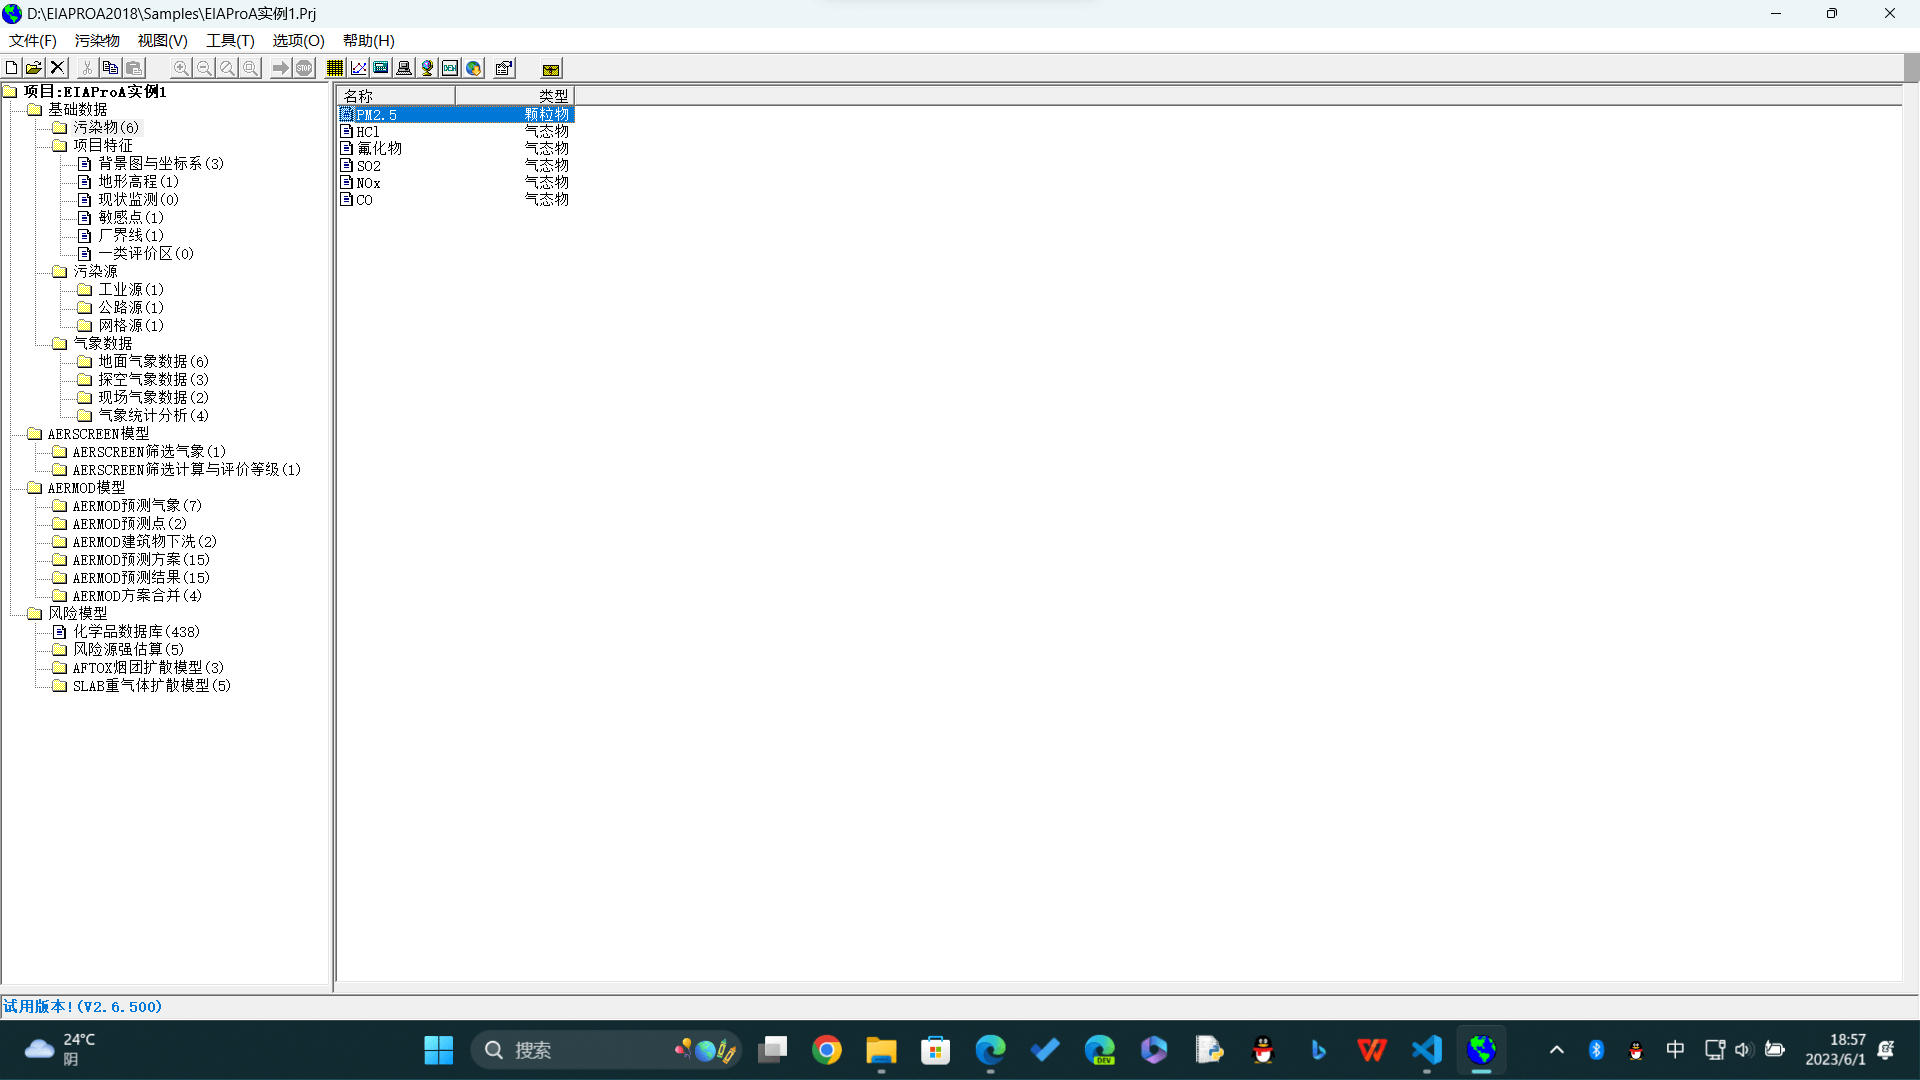
\includegraphics[width=0.8\textwidth]{figures/step1.png}
        \caption{输入境空气污染物浓度限值}
    \end{figure}
    \item 基础数据 $\rightarrow $ 项目特征 $\rightarrow $ 背景图与坐标系
    \begin{enumerate}[label=(\arabic*)]
        \item 插入城市生活垃圾环保发电厂(成都九江环保发电有限公司)的奥维互动地图——世纪空间卫星影像图;
        \item 红点的经纬度为 $(\text{经度}:103^{\circ}56'3.79'', \quad\text{纬度}:30^{\circ}38'32.18'')$;
        \item 图钉的经纬度为 $(\text{经度}:103^{\circ}56'9.18'', \quad\text{纬度}:30^{\circ}38'29.53'')$;
        \item 两者间相164.28 m,角度为$119.6^{\circ}$。
    \end{enumerate}
    \begin{figure}[H]
        \centering
        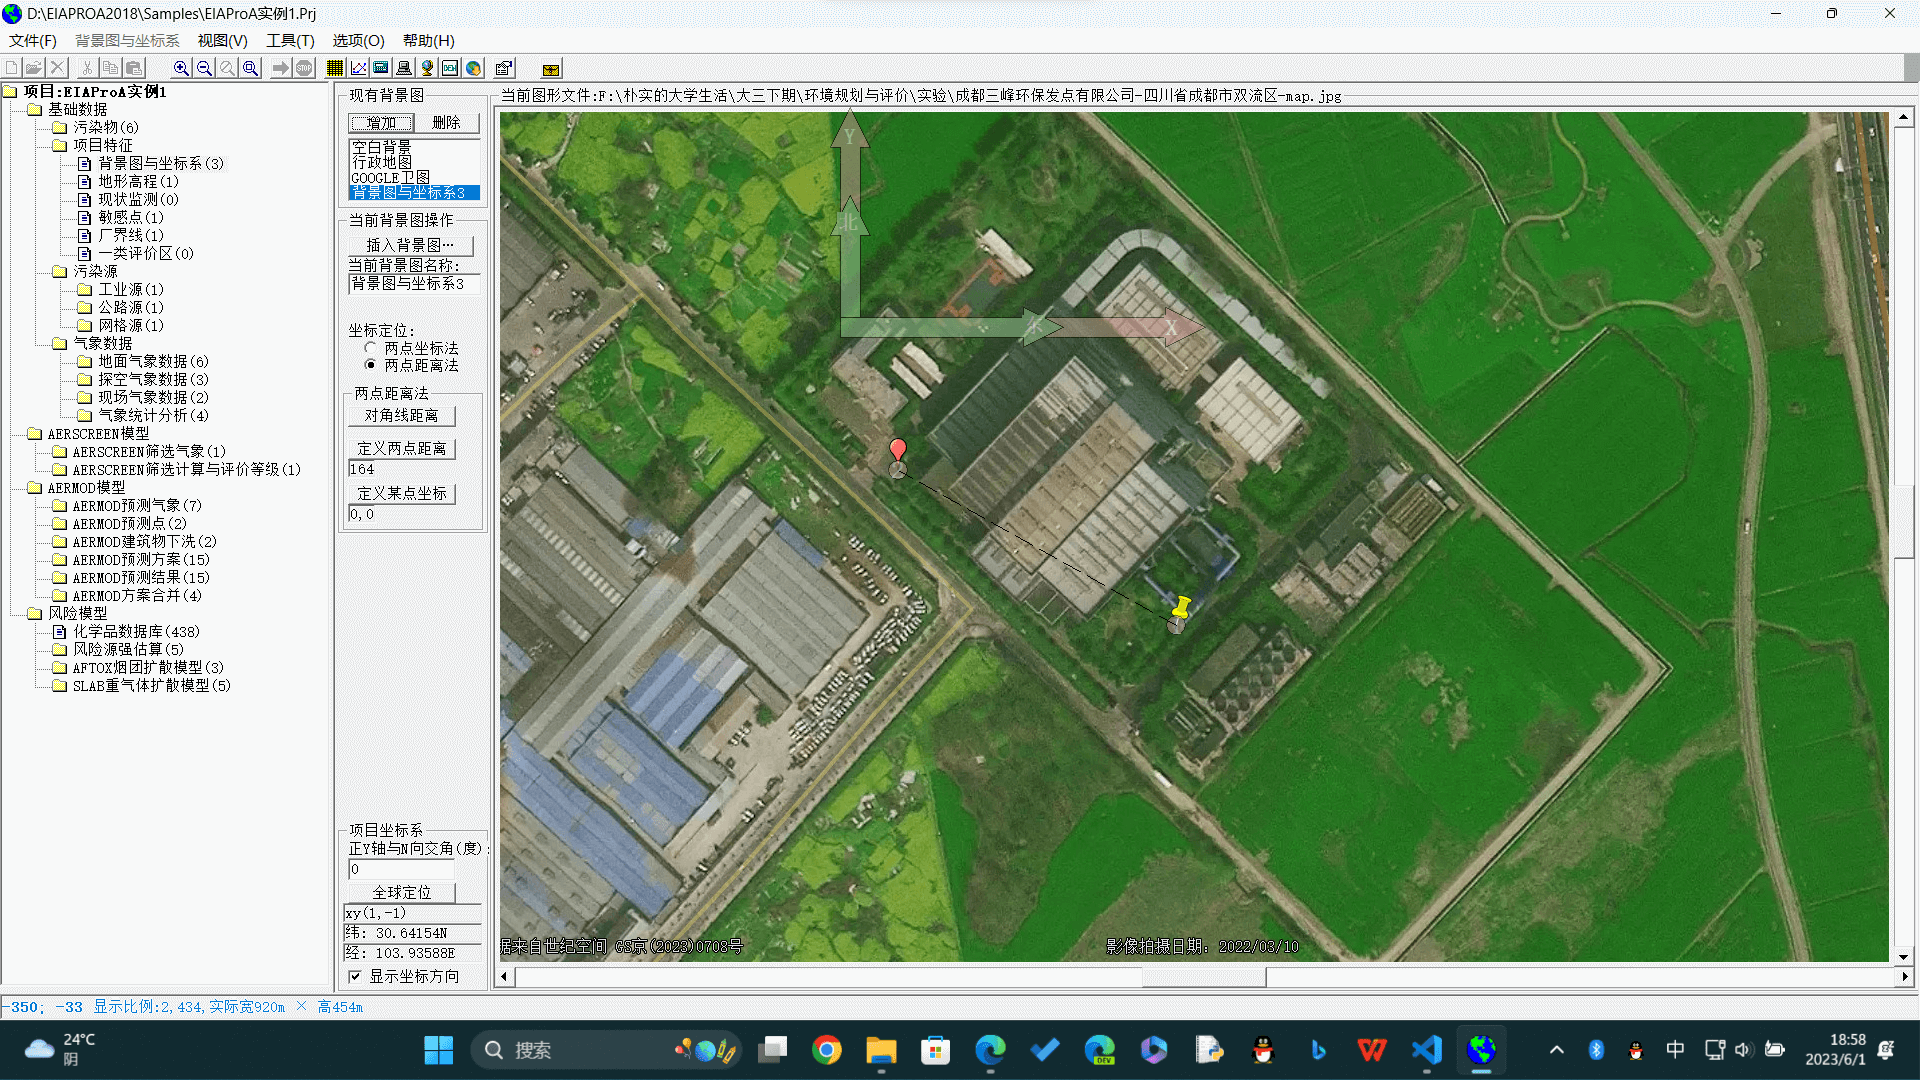
\includegraphics[width=0.8\textwidth]{figures/step2.png}
        \caption{插入项目卫星影像图}
    \end{figure}
    \item 基础数据 $\rightarrow $ 项目特征 $\rightarrow $ 地形高程 \\
    根据软件提示,手动配置一个“设为50*50 km范围”的DEM文件:
    \begin{figure}[H]
        \centering
        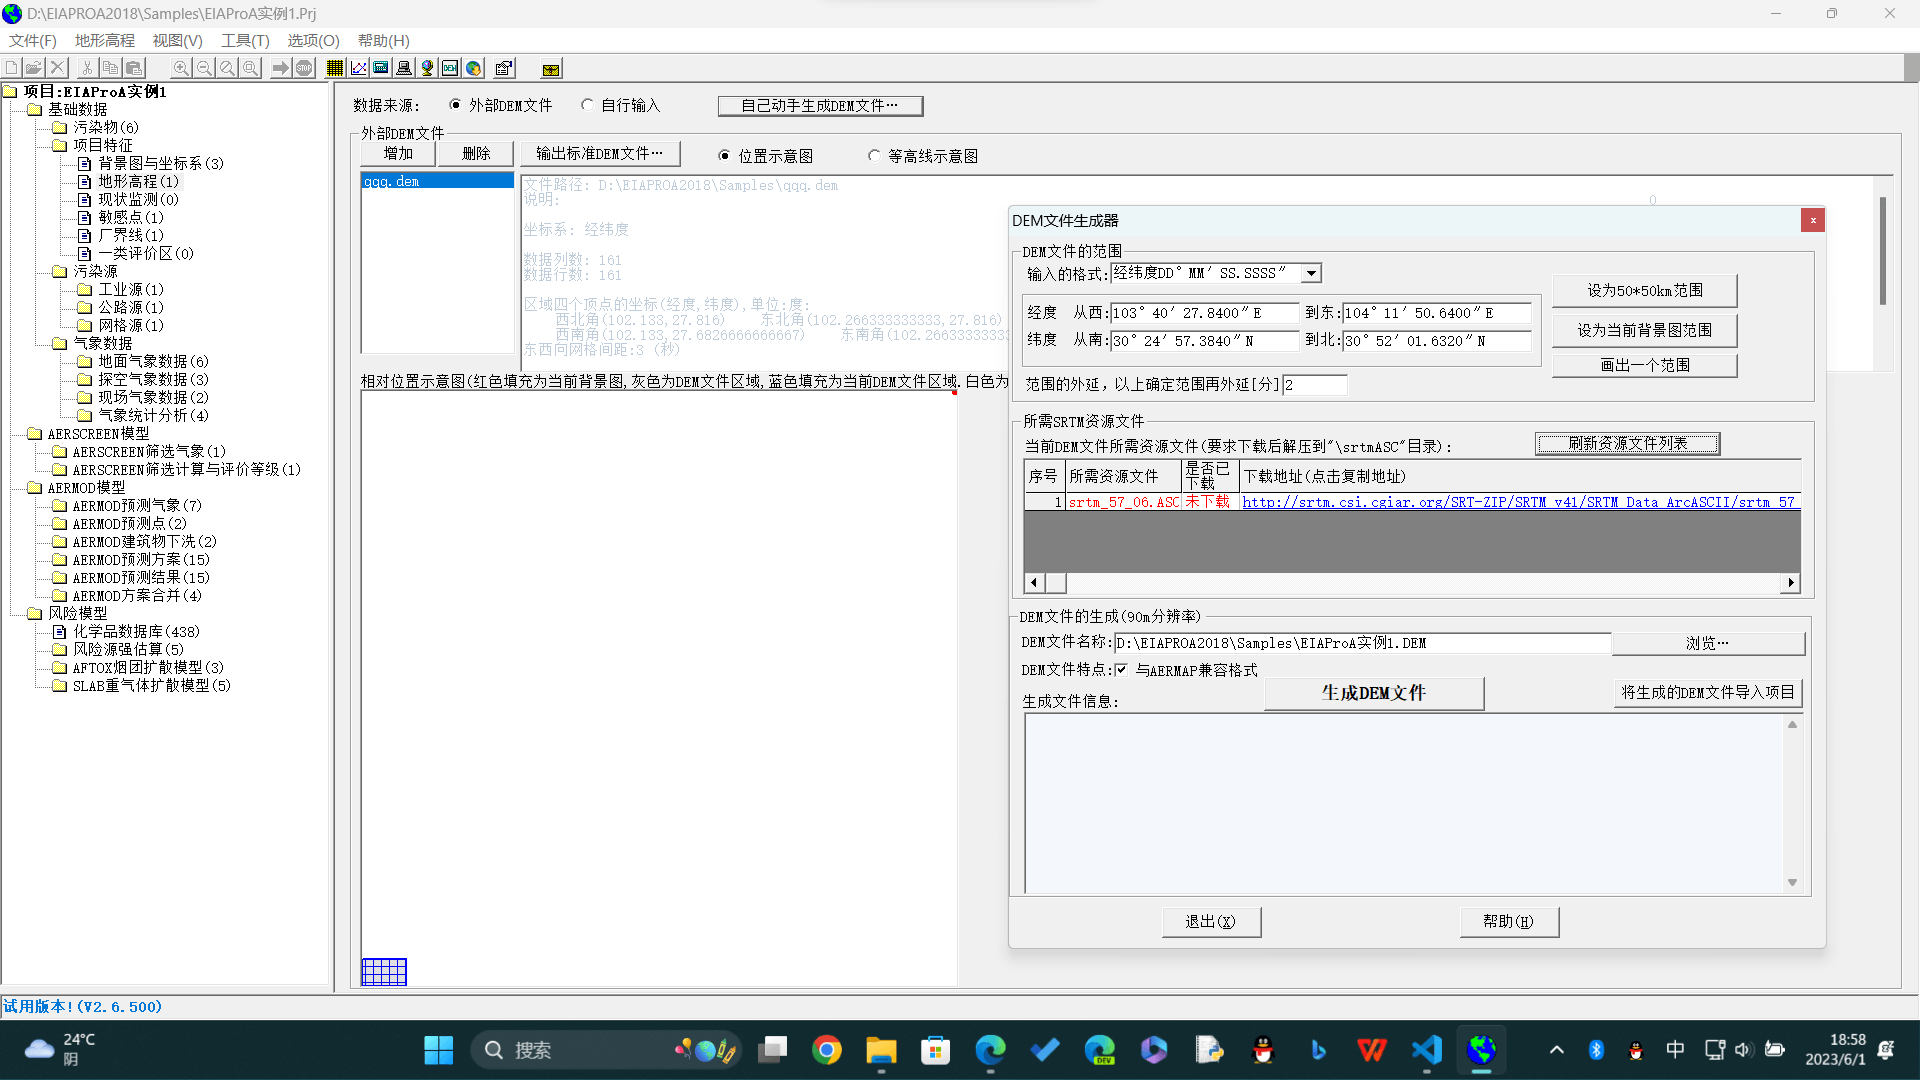
\includegraphics[width=0.8\textwidth]{figures/step3.png}
        \caption{配置添加DEM文件}
    \end{figure}
    \item 基础数据 $\rightarrow $ 污染源 $\rightarrow $ 工业源
    \begin{enumerate}[label=(\arabic*)]
        \item 选择污染物类型为点源;
        \item 根据污染源及项目周边条件基本信息(见表 \ref{tab:Basic information on pollution sources and surrounding conditions of the project}),填写:
        \begin{itemize}
            \item 烟筒几何高度: 130 m
            \item 烟筒出口内径: 5 m
            \item 输入烟气流量: 60000 Nm$^3$/h
            \item 出口烟气温度: $293-273.15=19.85$ ℃
        \end{itemize}
        \item 再根据污染物排放值(见表 \ref{tab:Pollutant emission value}),将污染物源强分别添入排放参数。
    \end{enumerate}
    \begin{figure}[H]
        \centering
        \begin{subfigure}[htpb]{0.8\textwidth}
            \centering
            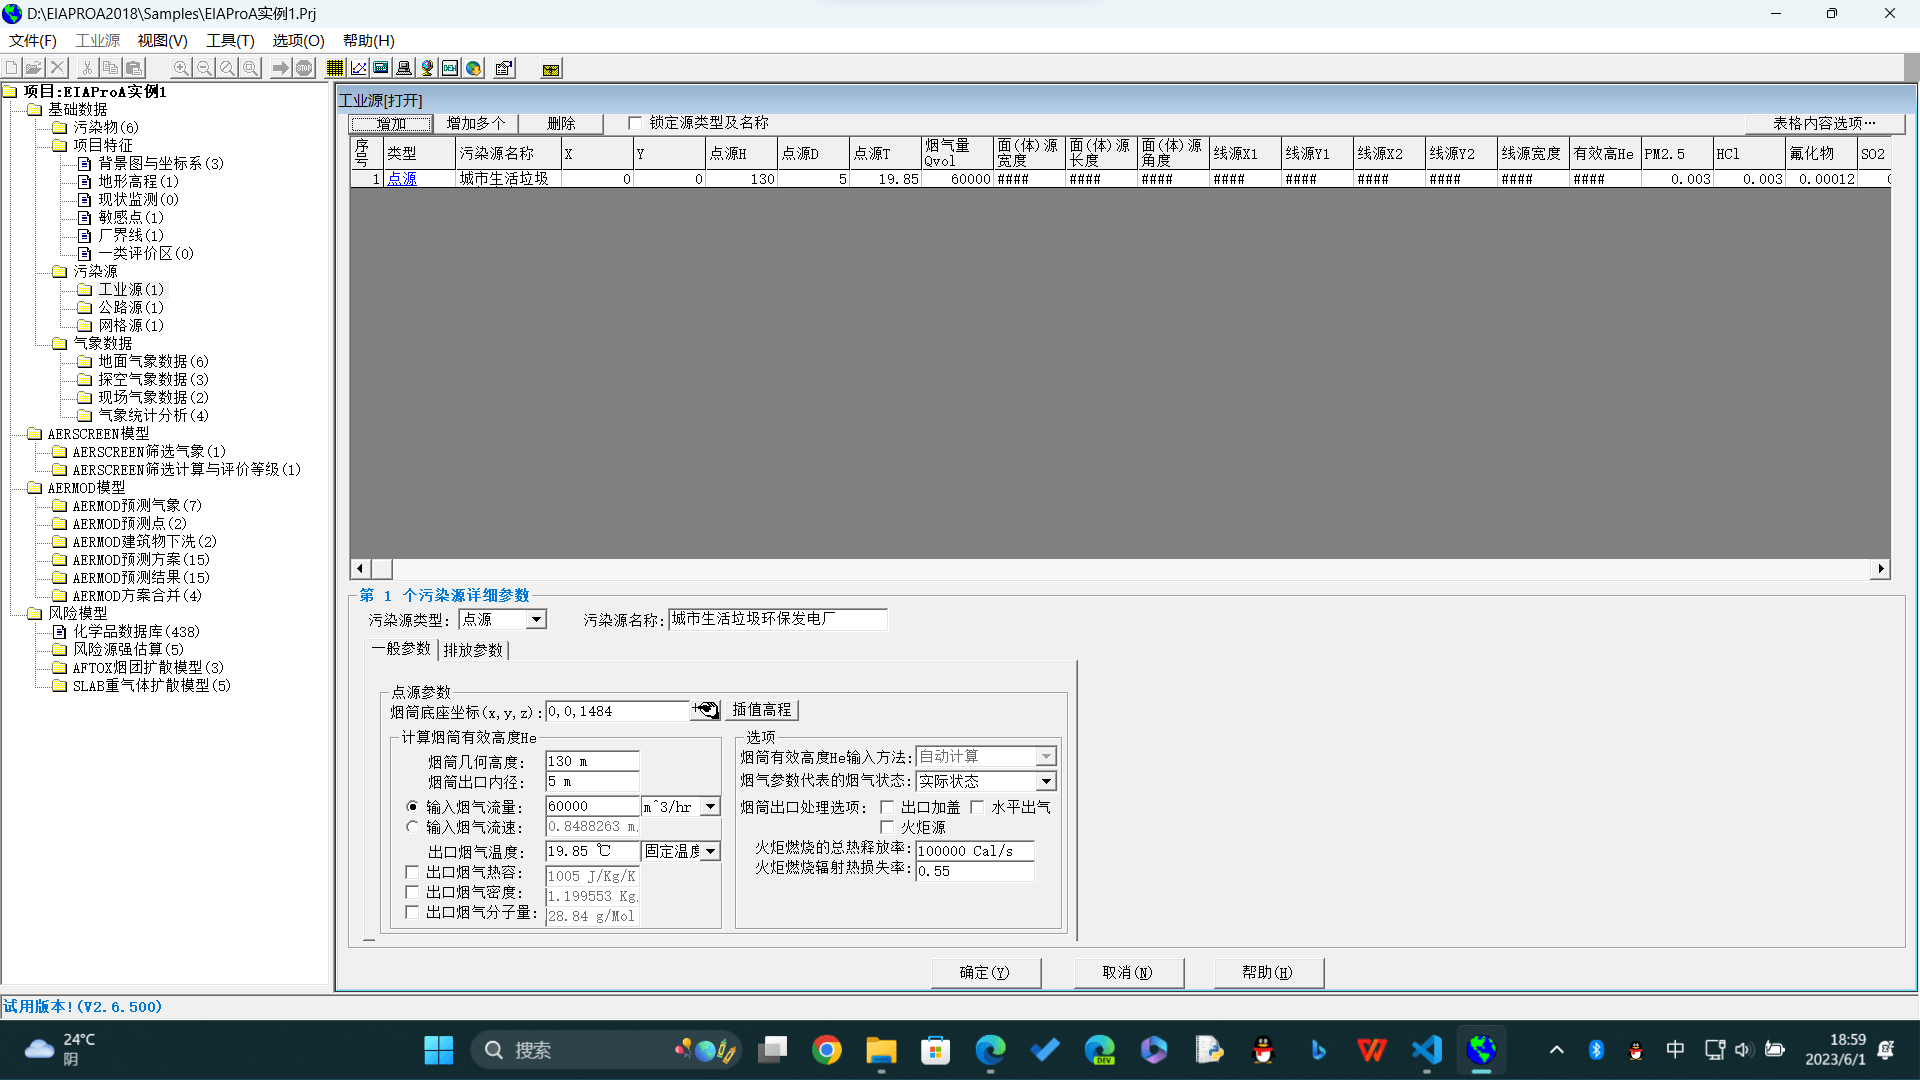
\includegraphics[width=\textwidth]{figures/step4-1.png}
            \caption{填写污染源一般参数}
        \end{subfigure}
        \quad
        \begin{subfigure}[htpb]{0.8\textwidth}
            \centering
            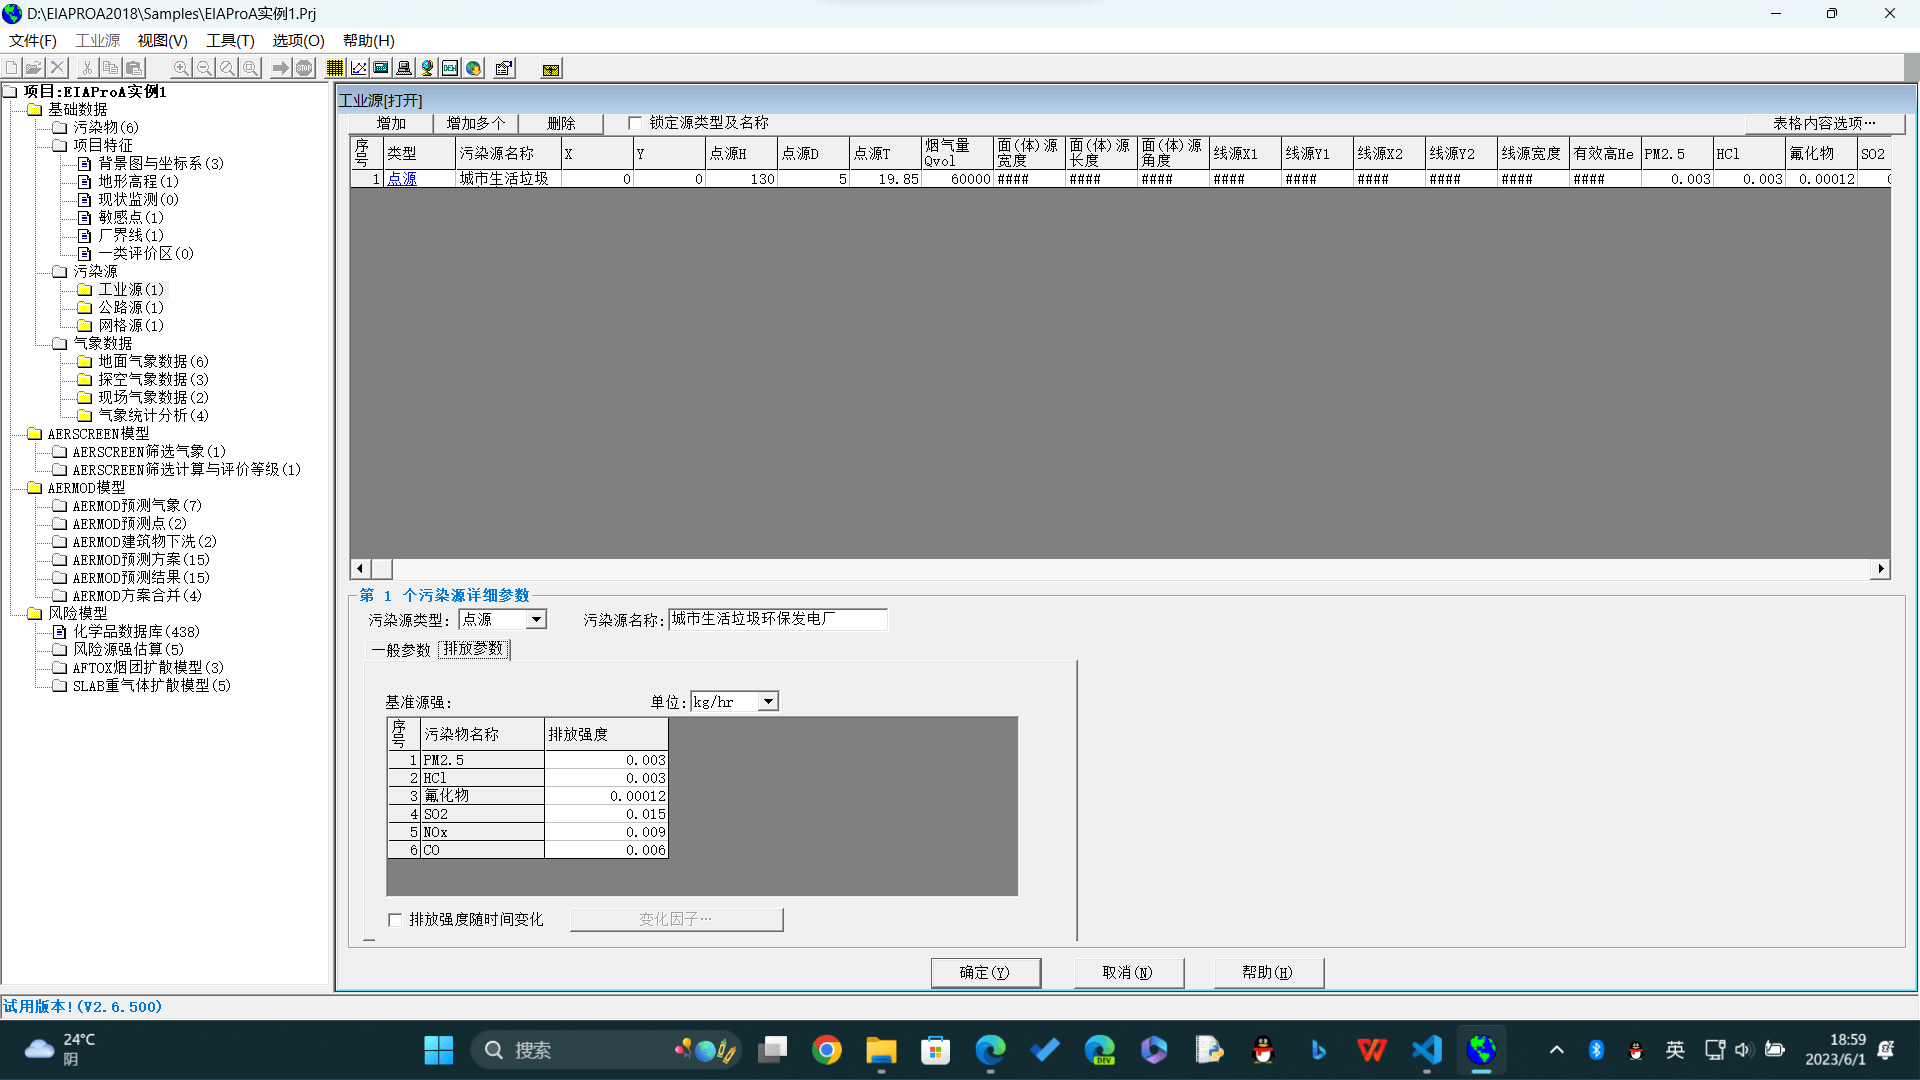
\includegraphics[width=\textwidth]{figures/step4-2.png}
            \caption{填写污染物排放参数}
        \end{subfigure}
        \caption{输入污染源信息}
    \end{figure}
    \item AERSCREEN模型 $\rightarrow $ AERSCREEN筛选气象
    \begin{enumerate}[label=(\arabic*)]
        \item 据污染源及项目周边条件基本信息(见表 \ref{tab:Basic information on pollution sources and surrounding conditions of the project}),填写:
        \begin{itemize}
            \item 项目所在地气温纪录最低: -6 ℃
            \item 项目所在地气温纪录最高: 44 ℃
            \item AERMET 通用地表类型: 城市
            \item AERMET 通用地表湿度: 潮湿气候
        \end{itemize}
        \item 查阅《环境影响评价技术导则——大气环境》(HJ 2.2-2018),估算模型 AERSCREEN :
        \begin{itemize}
            \item 最小风速可取 0.5 m/s
            \item 风速计高度取 10 m
        \end{itemize}
        \item 最后点击“生成特征参数表”。
    \end{enumerate}
    \begin{figure}[H]
        \centering
        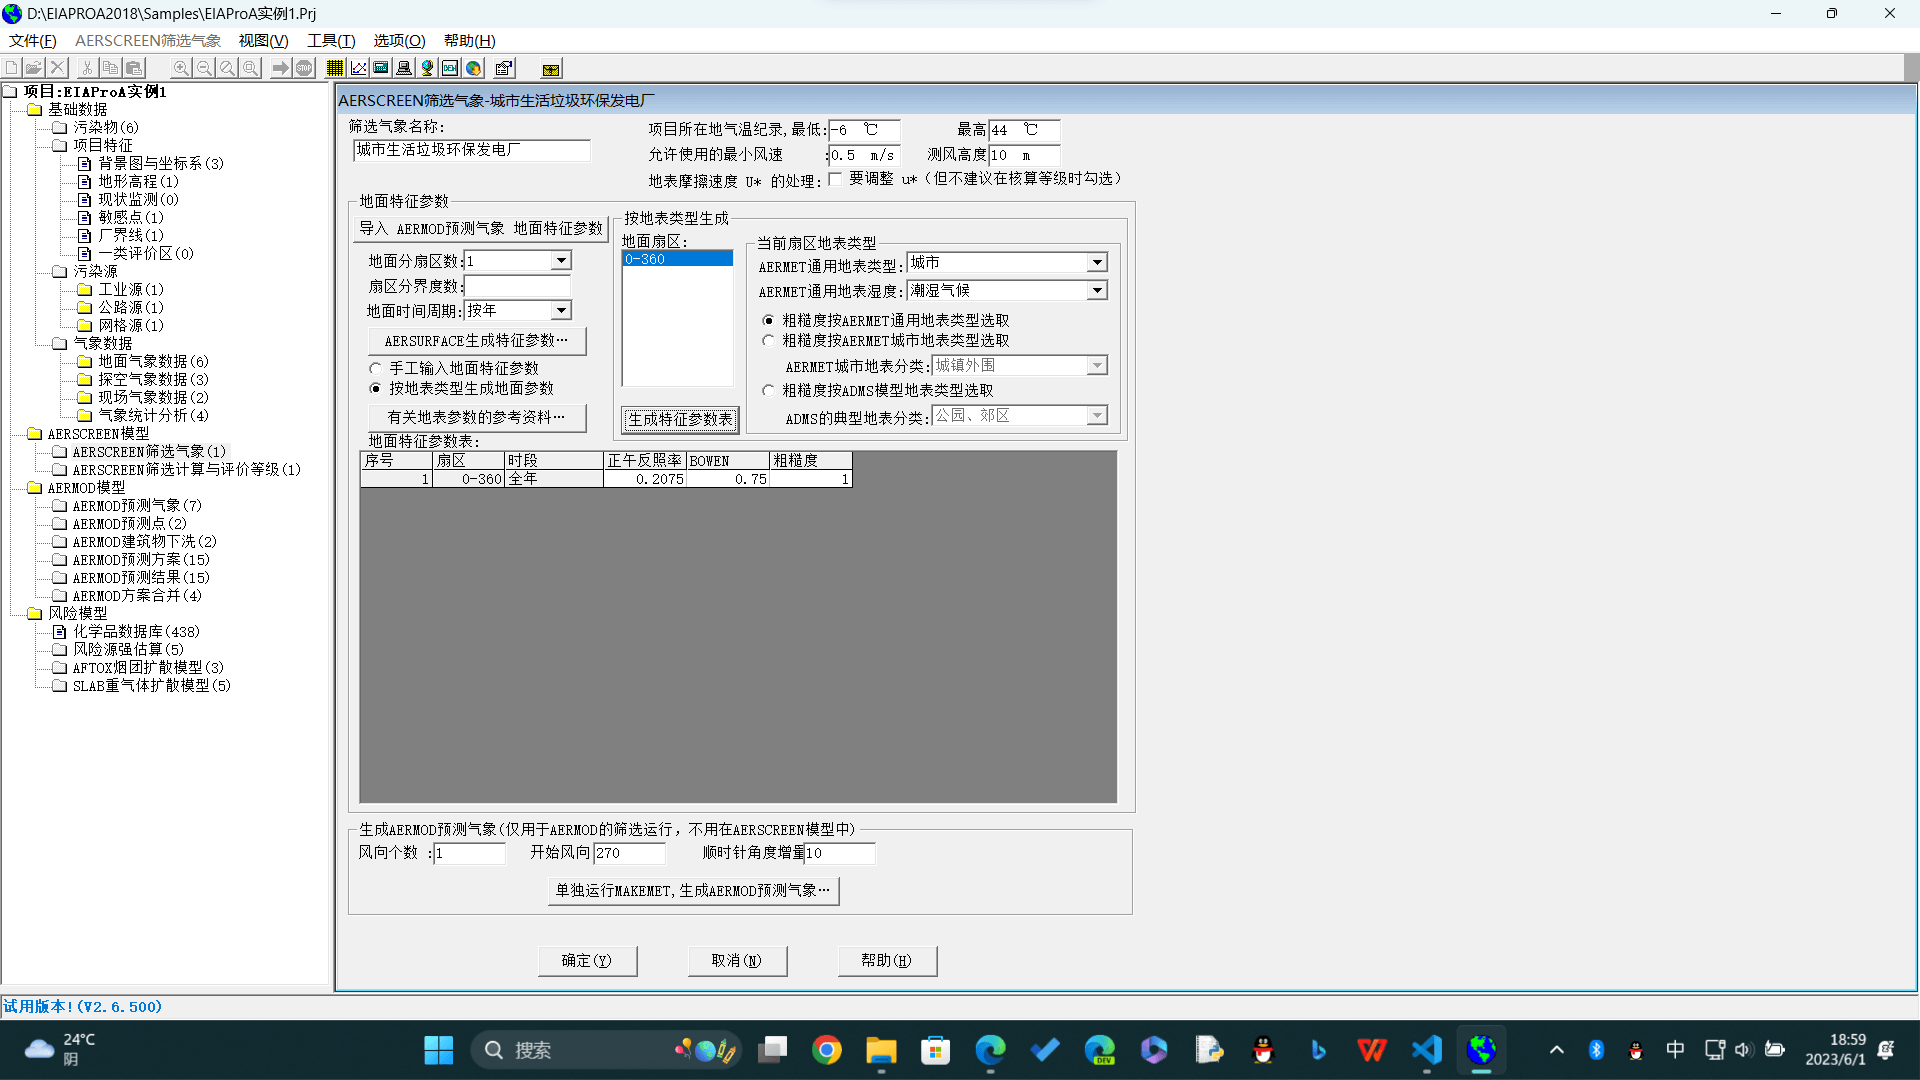
\includegraphics[width=0.8\textwidth]{figures/step5.png}
        \caption{输入筛选气象信息}
    \end{figure}
    \item AERSCREEN模型 $\rightarrow $ AERSCREEN筛选计算与评价等级
    \begin{enumerate}[label=(\arabic*)]
        \item 选择之前设定好的污染源和污染物参数(因为一个预测方案污染物个数限制为3,所以需要多次重复选取操作);
        \item 查阅《环境影响评价技术导则——大气环境》(HJ 2.2-2018),估算模型 AERSCREEN:
        \begin{itemize}
            \item 起始计算距离: 10 m
            \item 最大计算距离: 25000 m
        \end{itemize}
        \item 项目位置设置为农村;
        \item 取消勾选:考虑地形高程影响;
        \item 切换“筛选结果”,并点击“刷新结果”,得到数据分析信息。
    \end{enumerate}
    \begin{figure}[H]
        \centering
        \begin{subfigure}[htpb]{0.8\textwidth}
            \centering
            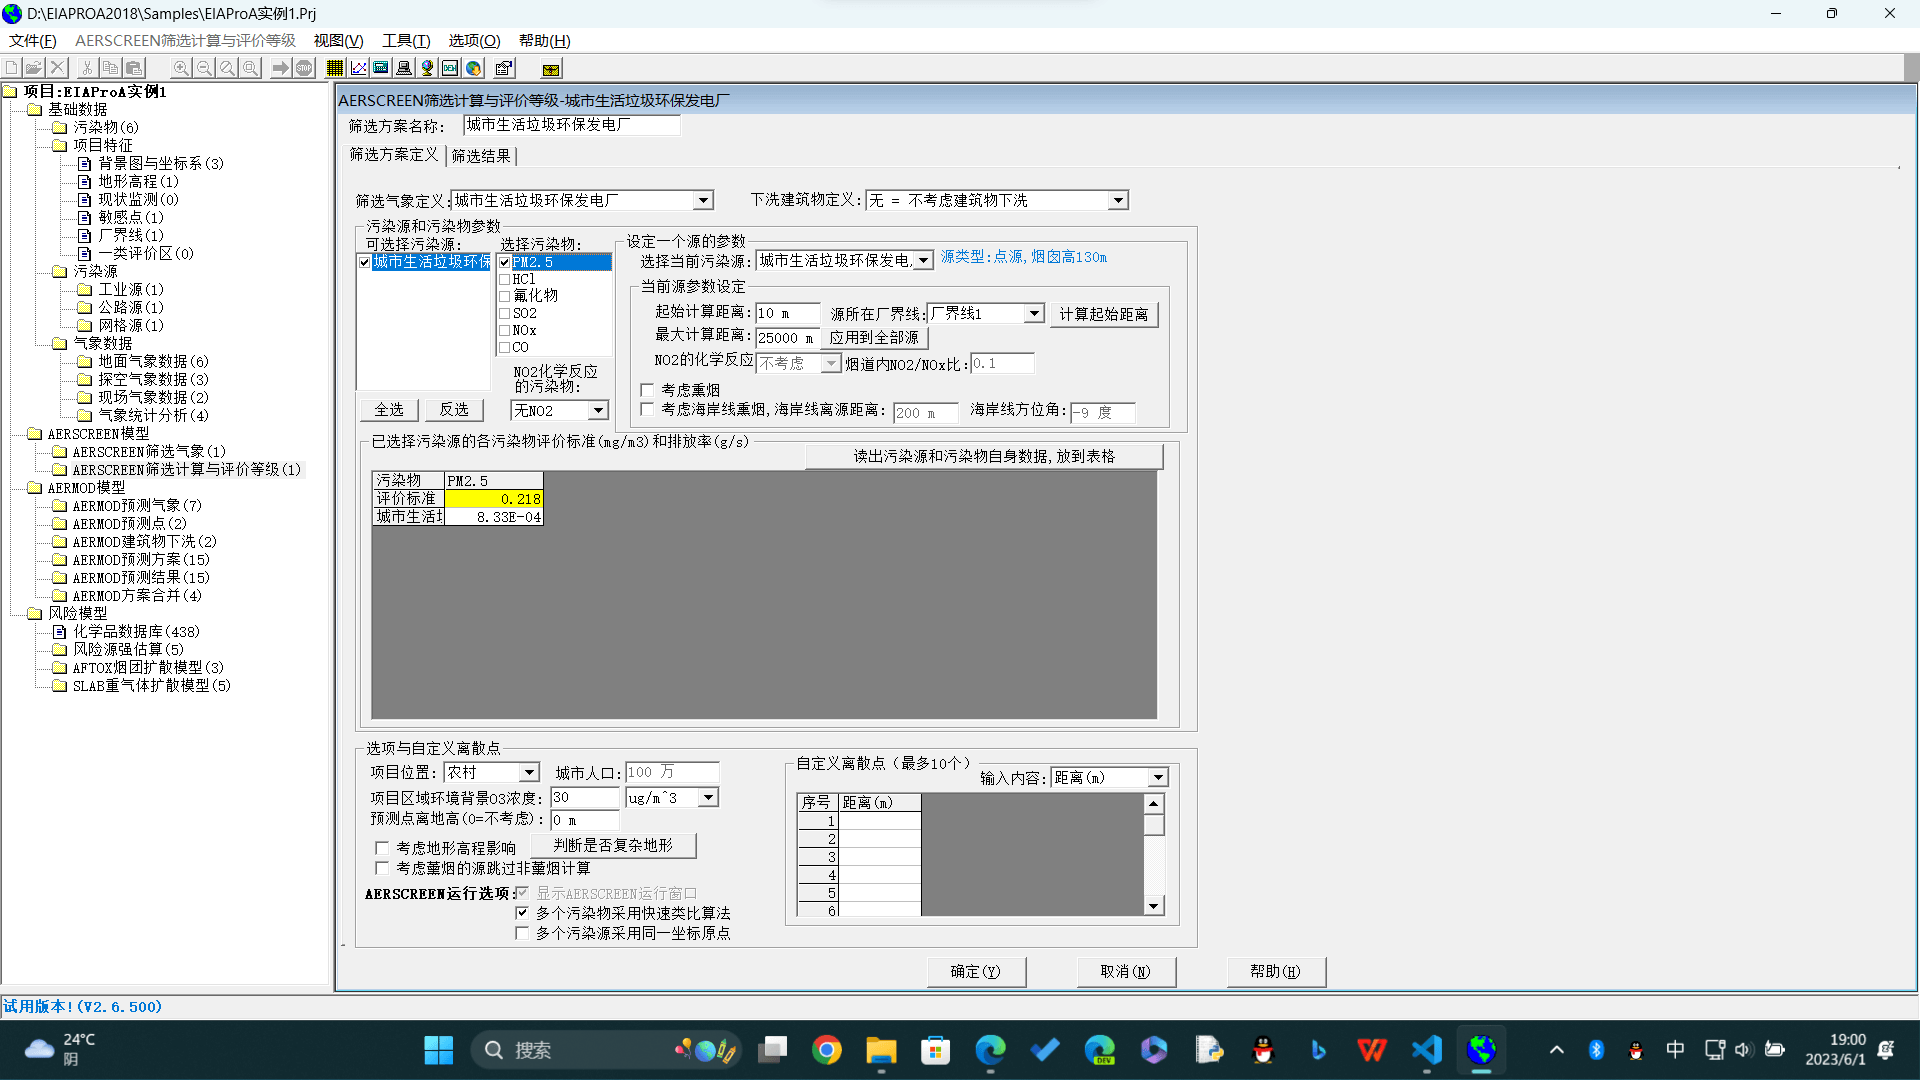
\includegraphics[width=\textwidth]{figures/step6-1.png}
            \caption{定义筛选方案}
        \end{subfigure}
        \quad
        \begin{subfigure}[htpb]{0.8\textwidth}
            \centering
            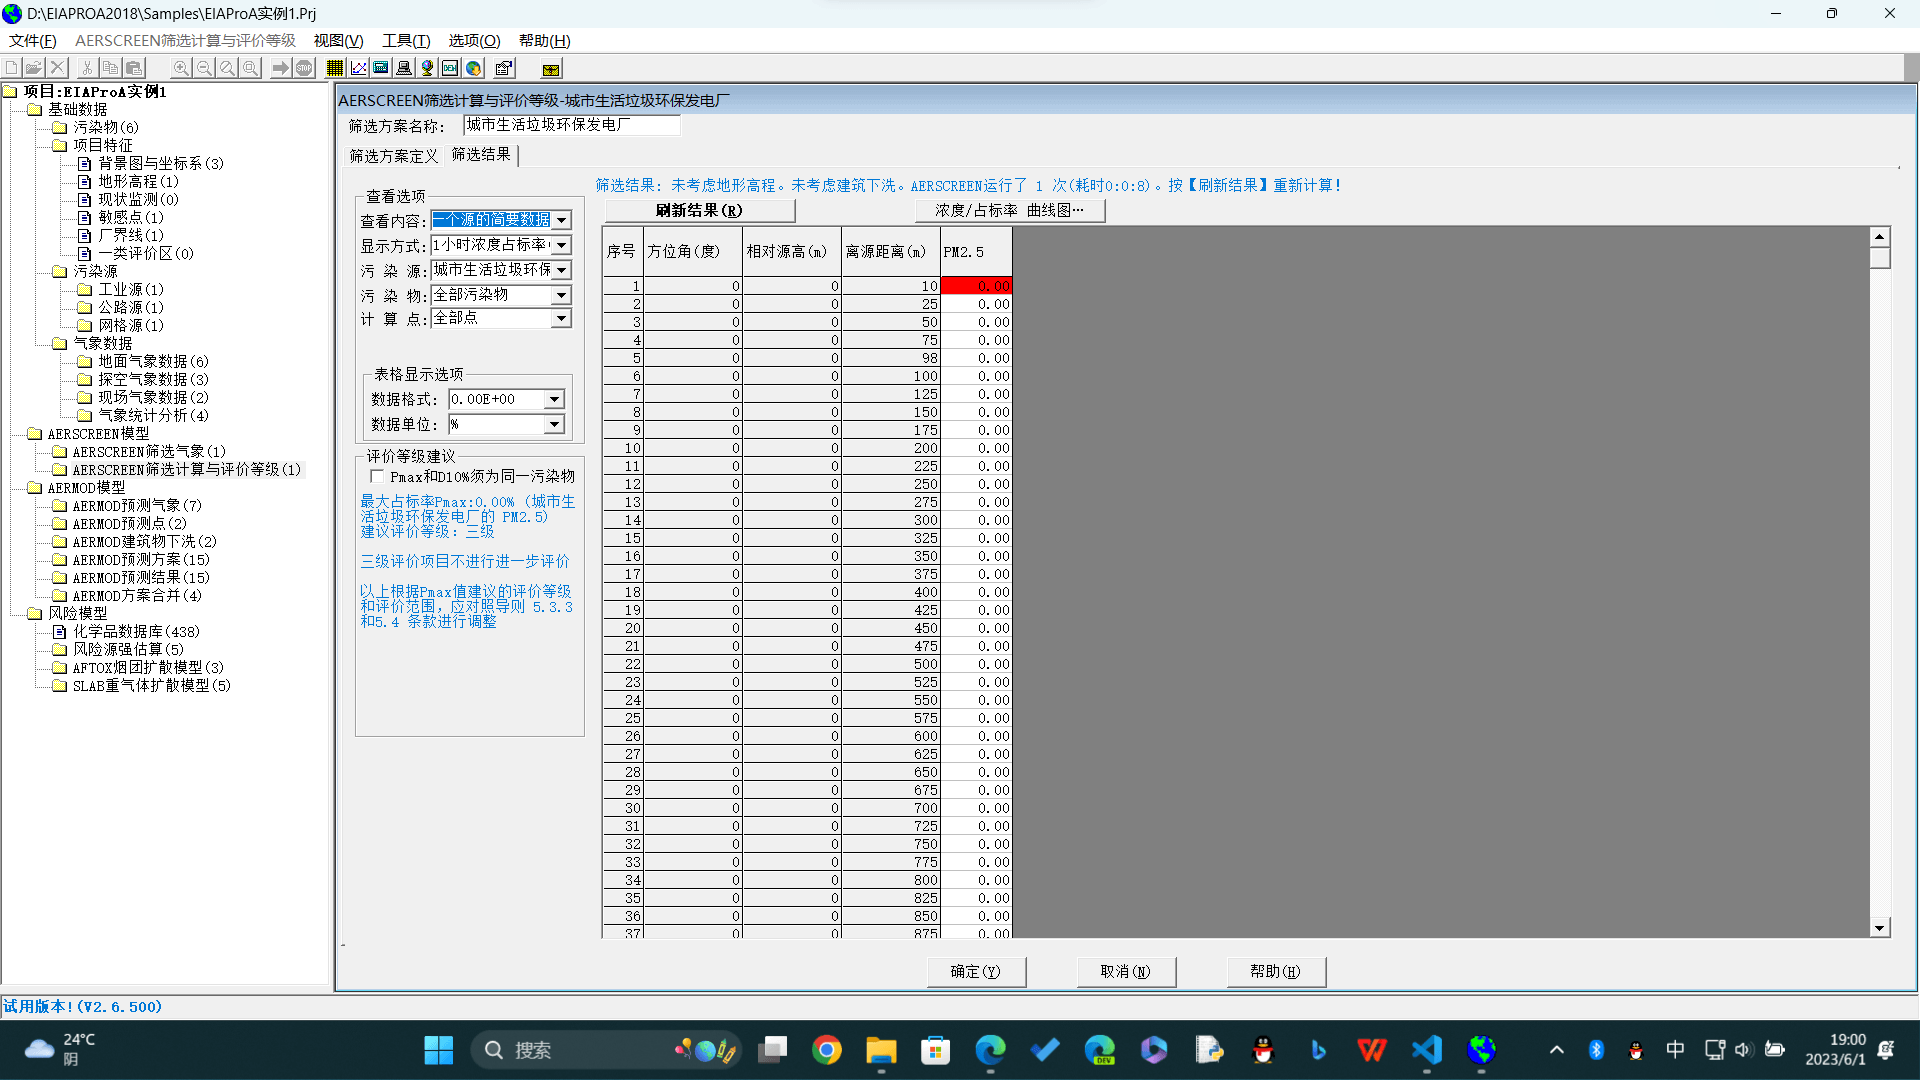
\includegraphics[width=\textwidth]{figures/step6-2.png}
            \caption{刷新筛选结果}
            \label{fig:Filter the results}
        \end{subfigure}
        \caption{筛选计算与评价等级}
    \end{figure}
    \item 结果汇总,完成等级评价。
    \begin{table}[H]
        \centering
        \caption{AERSCREEN筛选计算与评价等级结果}
        \resizebox{\textwidth}{!}{
        \begin{tabular}{ccccc}
        \toprule
        污染物名称 & 污染源强(kg/h) & 1h平均浓度限制(μg/m$^3$) & $P_{\mathrm{max}}$ (\%)  & 评价工作等级 \\
        \midrule
        颗粒物   & 0.003  & 217.5 & 3.059034E-03 & 三级 \\
        HCl   & 0.003  & 50    & 1.330680E-02 & 三级 \\
        HF    & 0.00012  & 20    & 1.330600E-03 & 三级 \\
        SOx   & 0.015  & 500   & 6.654200E-03 & 三级 \\
        NOx   & 0.009  & 250   & 7.984400E-03 & 三级 \\
        CO    & 0.006  & 10    & 1.331000E-04 & 三级 \\
        \bottomrule
        \end{tabular}}
        \label{tab:AERSCREEN screens the results of the calculation and evaluation of the grade}%
    \end{table}%  
\end{enumerate}


\subsubsection{筛选计算与评价等级优化}

由于EIAPROA2018软件的性能优化机制,再加上1小时浓度占标率(\%)的结果很小(从表 \ref{tab:AERSCREEN screens the results of the calculation and evaluation of the grade} 计算结果$P_{\mathrm{max}}$可以看出),在软件输出1小时浓度占标率(\%)时会自动进行四舍五入处理,而不是以科学计数法(0.00E+00)的形式显示(如图 \ref{fig:Filter the results} 所示)。这种处理方式给后续根据数据绘制占标率曲线带来了一些困扰。因此,为了解决这个问题,采取了一种不同的方法。
在软件启动时修改了AERSCREEN.exe文件的内置参数,以单独获取原始数据(.out文件),并使用Python读取,协助生成各污染物1小时内最大浓度和占标率曲线,如下所示:

\begin{figure}[H]
    \centering
    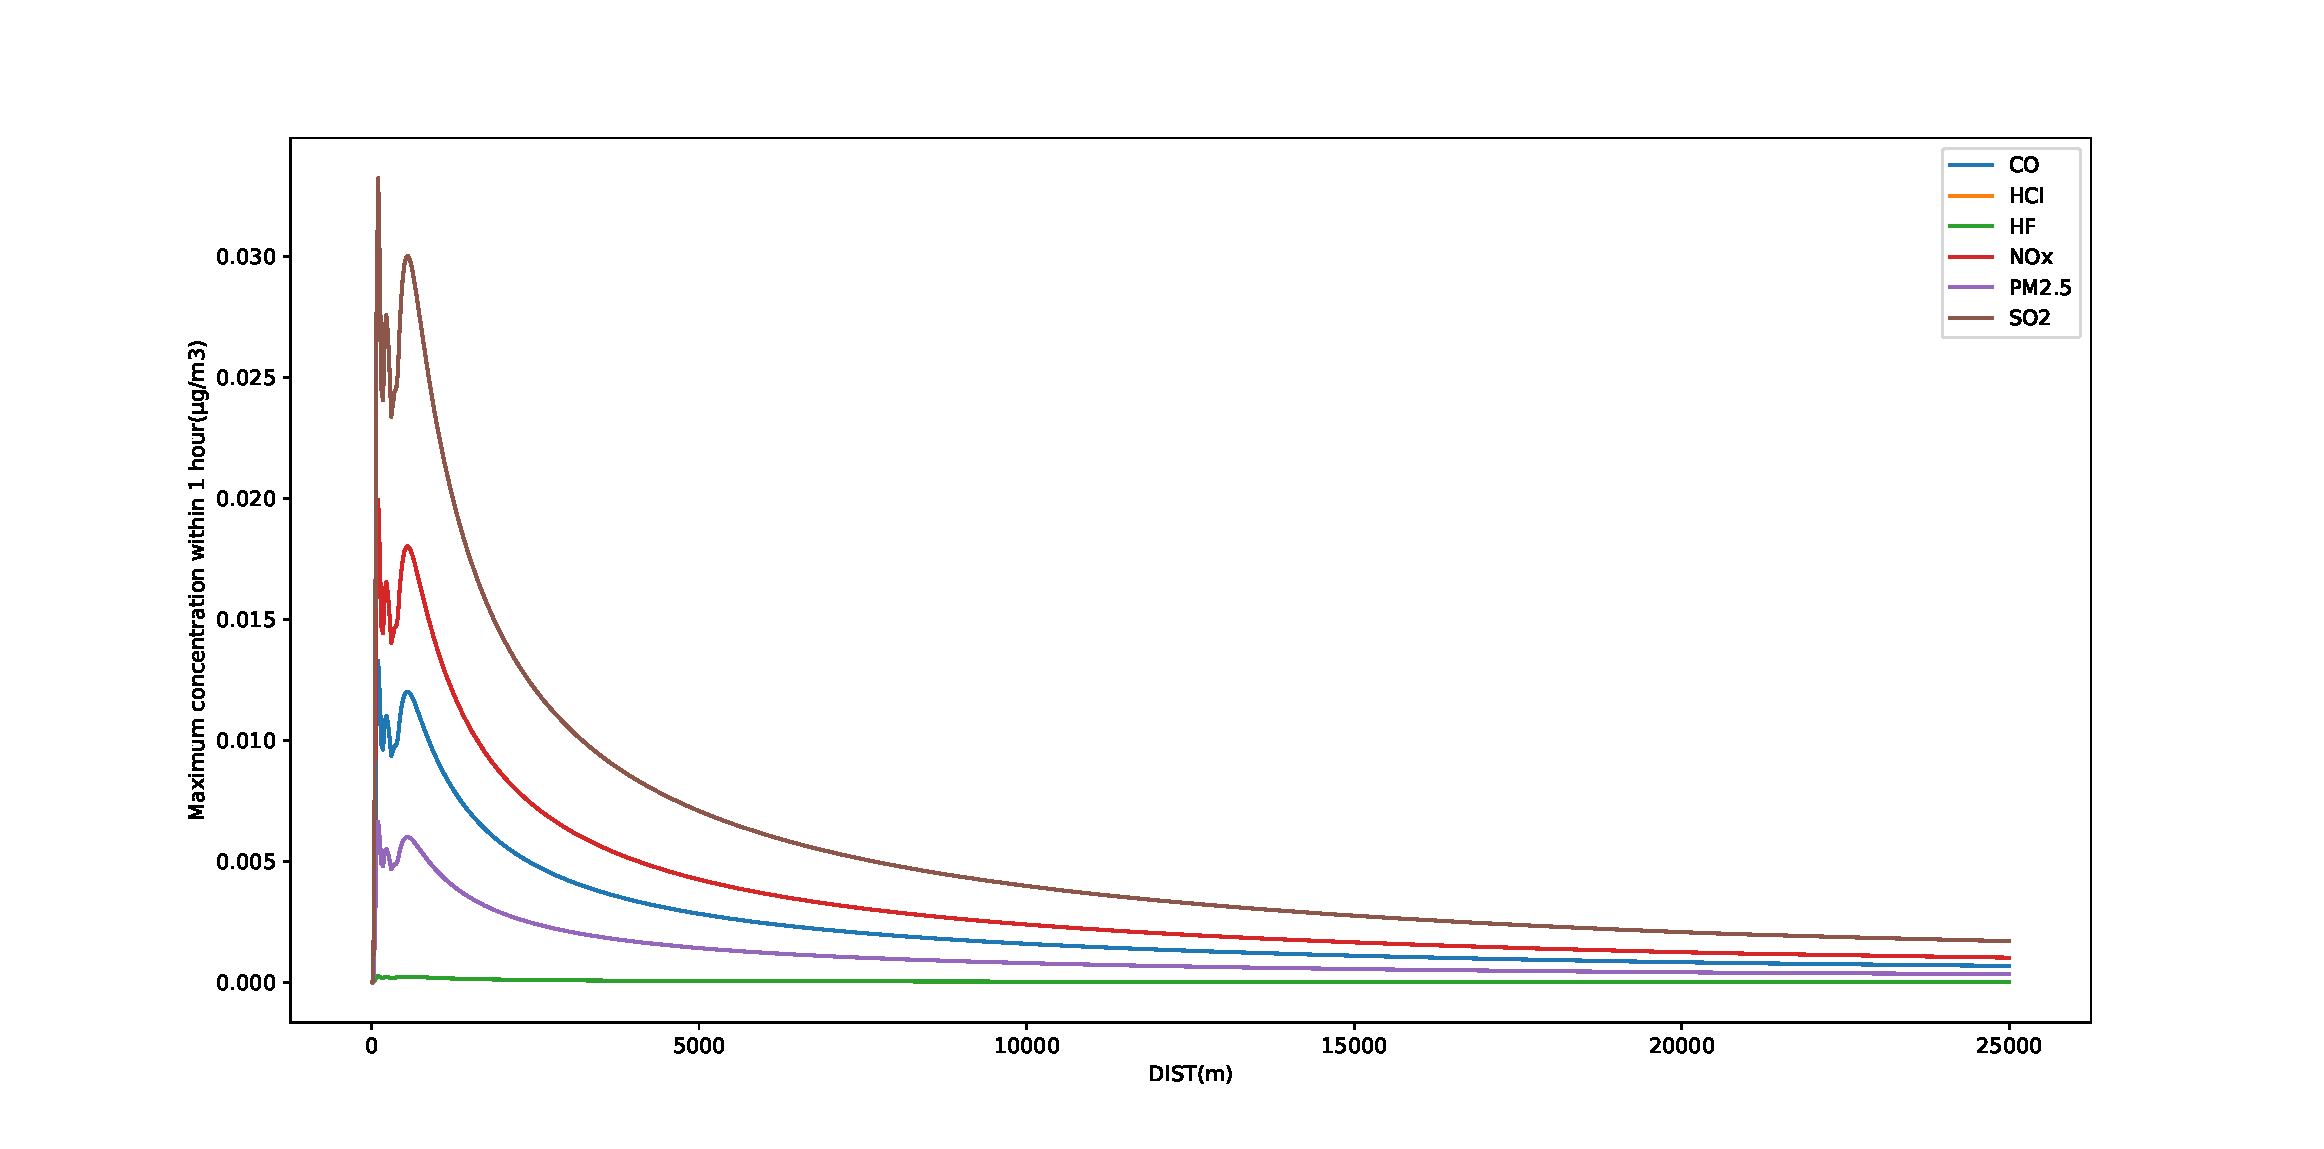
\includegraphics[width=\textwidth]{figures/Maximum concentration within 1 hour.pdf}
    \caption{各污染物1小时内最大浓度曲线}
    \label{fig:Maximum concentration within 1 hour}
\end{figure}
\noindent\textbf{注:}因为污染源强$\text{PM2.5}=\text{HCl}$,所以HCl的曲线被PM2.5的覆盖掉了。
\begin{figure}[H]
    \centering
    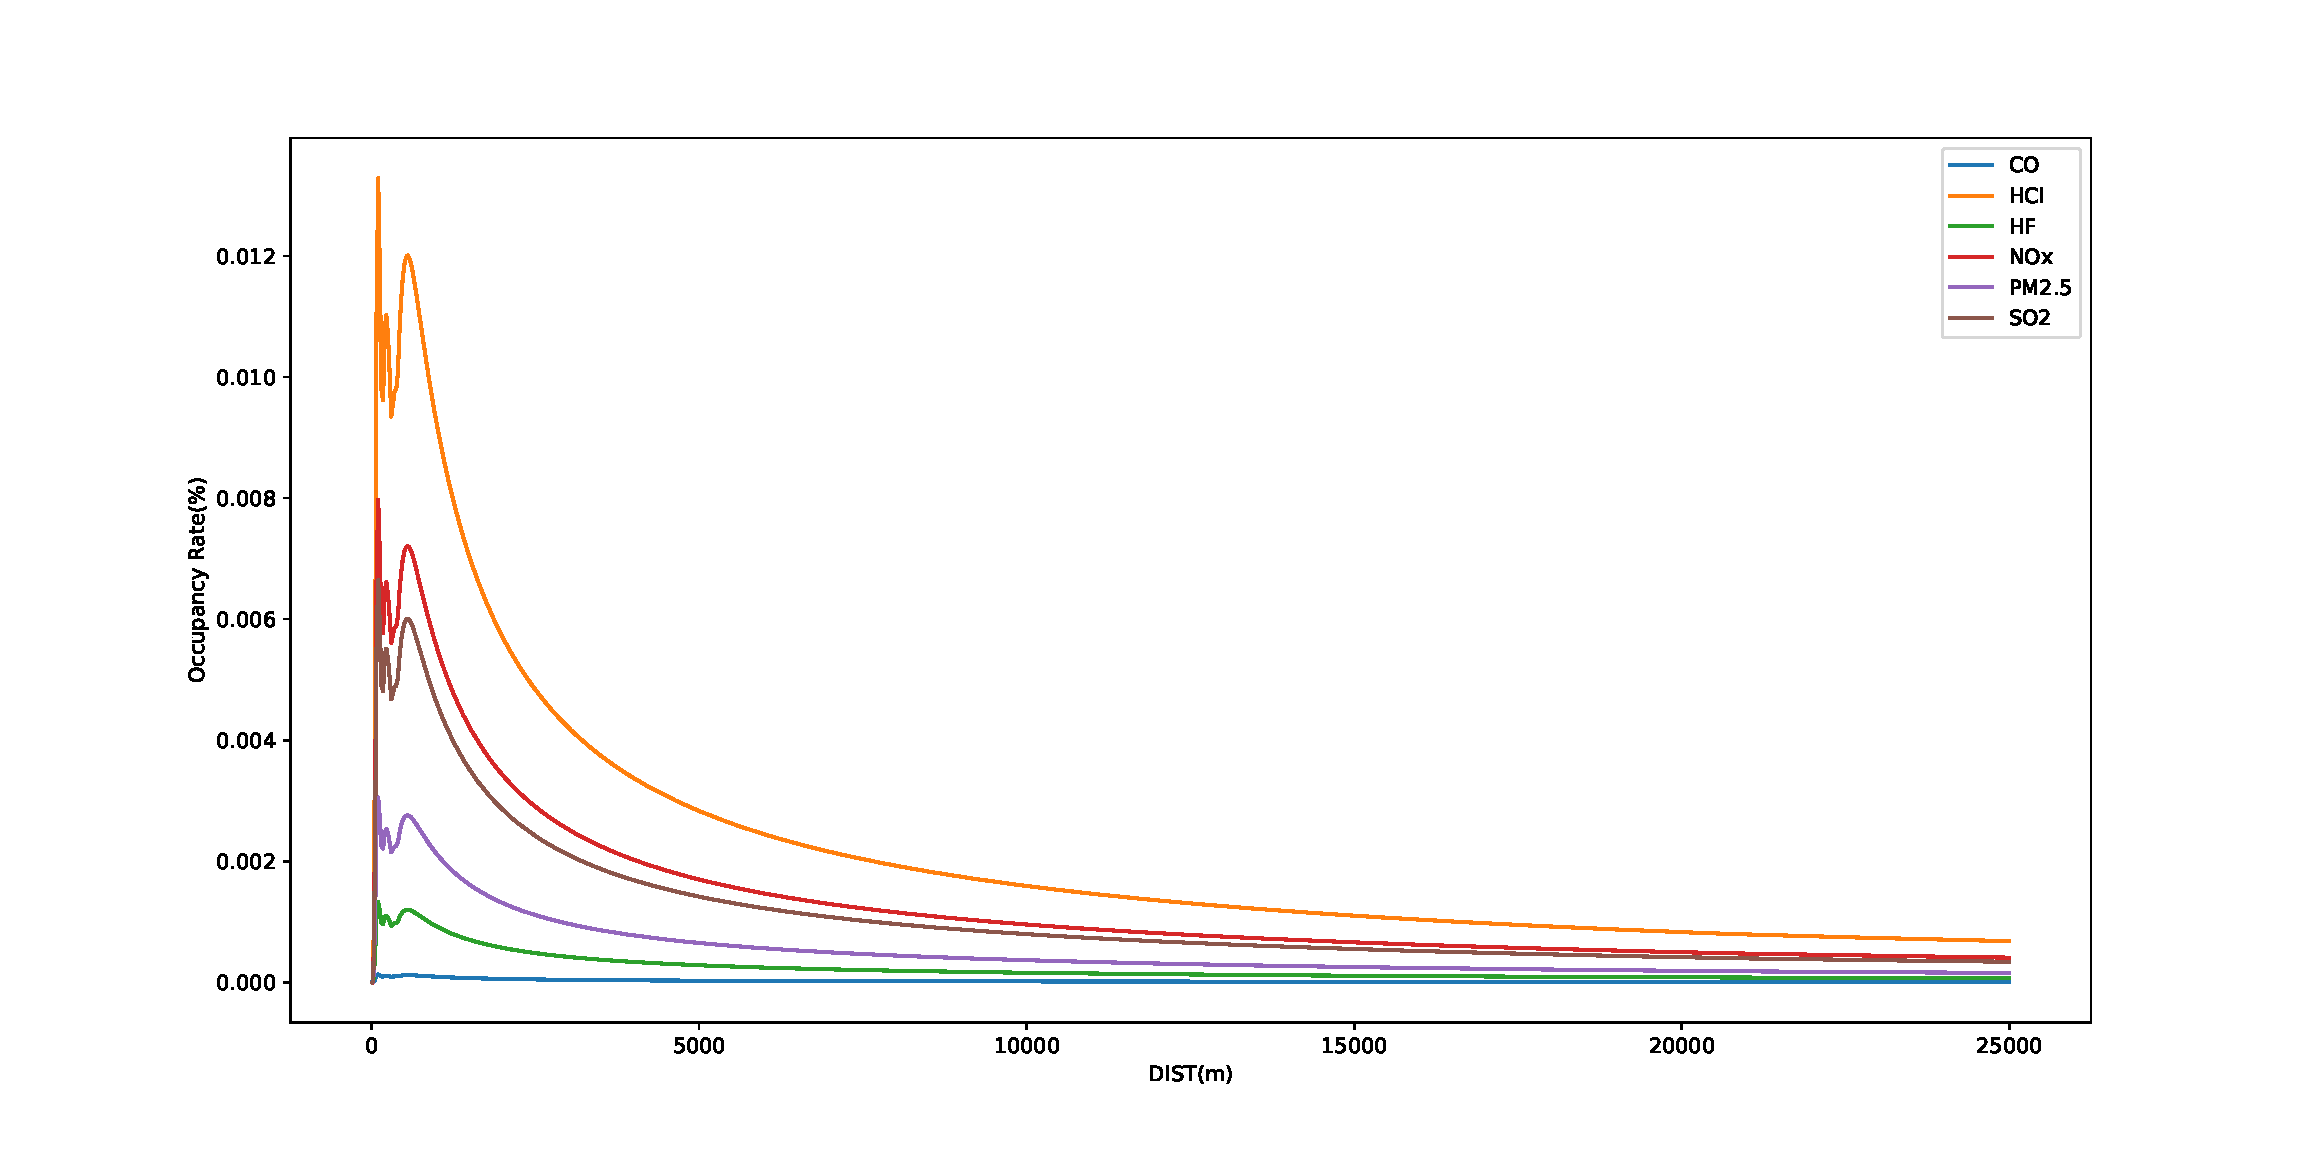
\includegraphics[width=\textwidth]{figures/1-hour concentration ratio curve.pdf}
    \caption{各污染物1小时浓度占标率曲线}
    \label{fig:1-hour concentration ratio curve}
\end{figure}


\subsubsection{大气环境监测计划}
成都市地处亚热带季风气候区,热量充足,雨量丰富,四季分明,雨热同期。除西北边缘部分山地以外,成都市大部分地区表现出的气候特点是:夏无酷暑,冬少冰雪,气候温和,夏长冬短,无霜期长,秋雨和夜雨较多,风速小,湿度大,云雾多,日照少。2021年,成都市年平均温度为$15.7\sim 18.0$℃;年极端最高气温为$36.1\sim 38.6$℃,年极端最低气温为$-1.7\sim -6$℃;最热月出现在7—8月,最冷月出现在1月。成都市年总降水量为$734.8\sim 1142.3$毫米,降水量总体偏多。成都市年平均日照时数为$843.9\sim 1406.2$小时。
\cite{成都气候特点}


\paragraph{$\bullet$ 监测范围}~{}\par
虽然三级评价项目不需设置大气环境影响评价范围\cite{HJ2.2-2018},但我们考虑到周边存在敏感点的实际情况(厂址左侧有工业厂区和居民区,右侧有高速公路),因此在本次大气环境监测计划中划定了一个以规划区边界为起点,并向外延伸2公里的区域作为整体的监测范围(见图 \ref{fig:Monitoring range and distribution map})。

\begin{figure}[H]
    \centering
    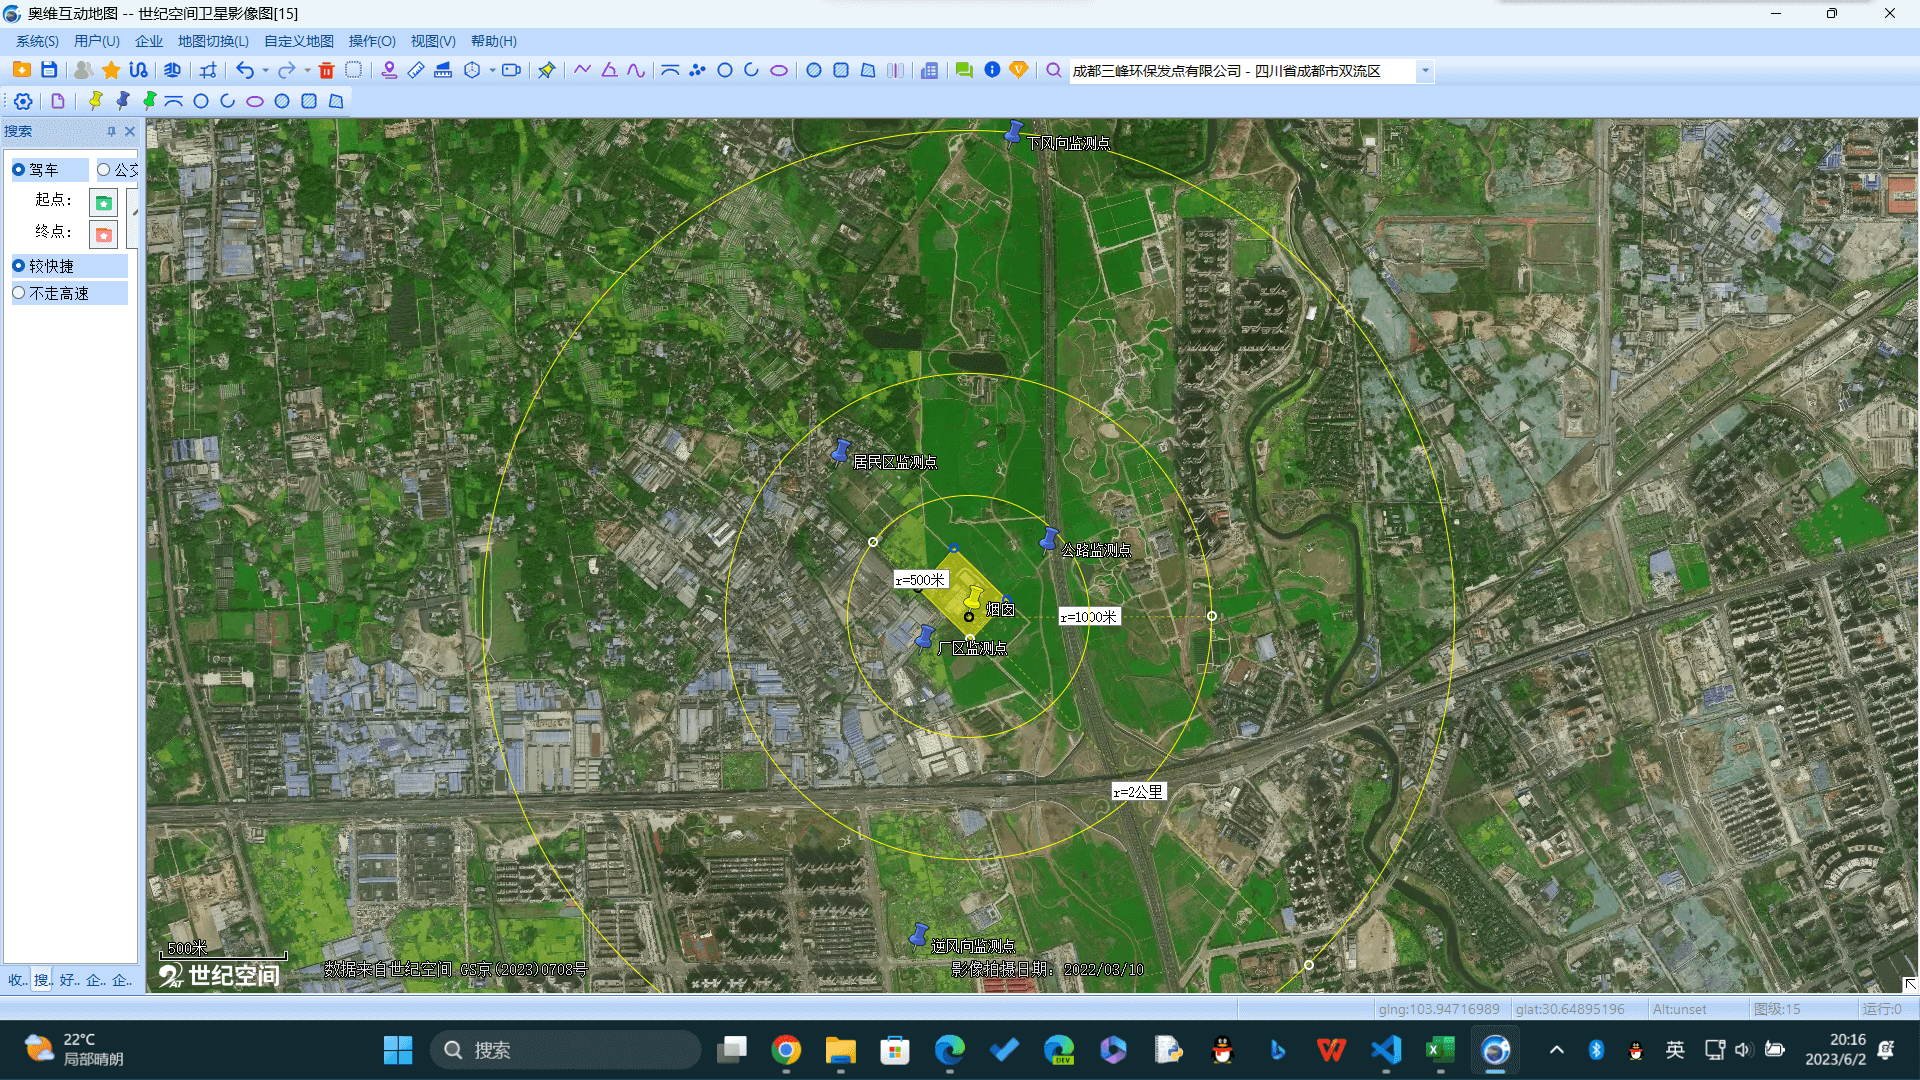
\includegraphics[width=\textwidth]{figures/Monitoring range and distribution map.png}
    \caption{监测范围及布点}
    \label{fig:Monitoring range and distribution map}
\end{figure}


\paragraph{$\bullet$ 监测布点}~{}\par

\begin{sidewaystable}[htbp]
    \centering
    \caption{监测点基本信息}
    \resizebox{24cm}{!}{
    \begin{tabular}{llllllll}
    \toprule
    监测点名称 & 环境背景  & 位置信息  & 监测目的  & 监测参数  & 监测设备  & 监测记录频率  & 汇总报告周期 \\
    \midrule
    厂区监测点 & 工业厂区  & \makecell[l]{经度:$103^{\circ}56'1.63''$\\纬度:$30^{\circ}38'24.24''$} & 评估对工业生产的影响 & \makecell[l]{PM2.5、HCl、HF、\\ $\mathrm{SO_2}$、$\mathrm{NO_x}$、CO} & 空气质量监测仪器 & 每天    & 每周 \\
    公路监测点 & 高速公路附近 & \makecell[l]{经度:$103^{\circ}56'20.78''$\\纬度:$30^{\circ}38'37.40''$} & 评估对交通道路的影响 & PM2.5、$\mathrm{NO_x}$、CO & 空气质量监测仪器 & 每周    & 每月 \\
    居民区监测点 & 近点居民区 & \makecell[l]{经度:$103^{\circ}55'48.63''$\\纬度:$30^{\circ}38'49.07''$} & 评估对居民生活环境的影响 & PM2.5、$\mathrm{SO_2}$、$\mathrm{NO_x}$ & 空气质量监测仪器 & 每天    & 每周 \\
    下风向监测点 & 厂址下风向 & \makecell[l]{经度:$103^{\circ}56'15.29''$\\纬度:$30^{\circ}39'31.47''$} & 评估污染扩散程度 & PM2.5、$\mathrm{SO_2}$、$\mathrm{NO_x}$ & \makecell[l]{风向监测仪器\\空气质量监测仪器} & 每小时   & 每天 \\
    逆风向监测点 & 厂址逆风向 & \makecell[l]{经度:$103^{\circ}56'0.67''$\\纬度:$30^{\circ}37'44.73''$} & 评估污染扩散程度 & PM2.5、$\mathrm{SO_2}$、$\mathrm{NO_x}$ & \makecell[l]{风向监测仪器\\空气质量监测仪器} & 每小时   & 每天 \\
    \bottomrule
    \end{tabular}}
    \label{tab:Basic information about monitoring points}%
\end{sidewaystable}%

根据《环境影响评价技术导则——大气环境》(HJ 2.2-2018)的要求,在选择监测点时,应考虑当地主导风向以及厂址及主导风向下风向的范围。针对环境评价中的污染物,特别是PM2.5、HCl、HF、SO2、NOx和CO,我们根据成都市气象局公布的长期风向资料进行了综合分析。

据成都市气象局网站公布的《成都市常年各月风向、风速、降水气候资料》显示:成都市属亚热带湿润季风气候区,成都市常年最多风向是静风;次多风向:6、7、8 月为北风,其余各月为东北偏北风。基于这些信息,我们选择了两个监测点,分别位于厂址烟囱位置向北偏东一点的方向和厂址烟囱位置的反方向,以确保监测点能够覆盖主导风向和下风向范围。

此外,根据《环境影响评价技术导则——大气环境》(HJ 2.2-2018)的建议,环境质量监测点应该设置在项目厂界或大气环境防护距离外侧。考虑到厂区附近的工业厂区、居民区以及高速公路的存在,我们在500米和1000米范围内分别设置了三个额外的监测点。这样的安排旨在全面评估厂区对工业生成、交通道路和居民生活环境的影响,并评估污染物在不同方向上的扩散程度。

通过这样的监测点设置(见图 \ref{fig:Monitoring range and distribution map}、表 \ref{tab:Basic information about monitoring points}),我们能够全面了解环保发电厂产生的污染物对周围环境的影响,并及时监测和评估空气质量。监测设备将定期记录数据,根据监测频率进行数据汇总和报告,以确保及时了解大气环境的状况并采取必要的措施来保护环境和人们的健康。


\paragraph{$\bullet$ 监测因子} (PM2.5、HCl、HF、$\mathrm{SO_2}$、$\mathrm{NO_x}$、CO)

确定环境质量监测因子,我们需要筛选出按公式 \ref{eq:The maximum ground concentration of the pollutant is standardized} 要求计算的排放污染物 $P_i \geqslant 1\%$ 的项目。\cite{HJ2.2-2018} 然而,根据实际情况的需求,表 \ref{tab:AERSCREEN screens the results of the calculation and evaluation of the grade} 中的六种污染物都未达到 $P_{\mathrm{max}} \geqslant 1\% $ 的标准,因此不能单独作为环境质量监测因子。尽管如此,考虑到它们是项目监测中的常规监测因子,我们仍然将它们纳入了大气环境监测计划的环境质量监测因子范畴。


\paragraph{$\bullet$ 监测方法}~{}\par

根据所确定的六个监测因子(PM2.5、HCl、HF、$\mathrm{SO_2}$、$\mathrm{NO_x}$、CO),分别选择相应的分析监测方法,如下表 \ref{tab:Various monitoring factor analysis methods} 所示:
\begin{table}[H]
    \centering
    \caption{各项监测因子分析方法}
    \begin{tabular}{lll}
    \toprule
    监测因子 & 分析方法  & 方法来源 \\
    \midrule
    $\mathrm{SO_2}$   & 紫外荧光法、差分吸收光谱分析法 & GB 3095-2012 \\
    CO    & 气体滤波相关红外吸收法、非分散红外吸收法 & GB 3095-2012 \\
    $\mathrm{PM_{2.5}}$ & 微量振荡天平法、β射线法 & GB 3095-2012 \\
    $\mathrm{NO_x}$   & 化学发光法、差分吸收光谱分析法 & GB 3095-2012 \\
    HCl   & 离子色谱法 & HJ 549-2016 \\
    HF    & 滤膜采样/氟离子选择电极法 & HJ 955-2018 \\
    \bottomrule
    \end{tabular}%
    \label{tab:Various monitoring factor analysis methods}%
\end{table}%


\paragraph{$\bullet$ 监测时期}~{}\par
由于成都市位于亚热带湿润季风气候区,静风是该地区的主要风向。次之的是北风,主要出现在6、7、8月,而东北偏北风则是其他月份的主要风向。考虑到7-8月份是最炎热的季节,这段时间内污染物更容易朝北方扩散。因此,在监测时期的选择上,我们倾向于以夏季为主,同时也会考虑其他季节的情况。这样的选择有助于我们更全面地了解该厂址污染物的排放对周围环境质量影响的变化趋势。

夏季作为最热的季节,空气中的污染物浓度往往较高,因此监测这一时期的数据可以提供关于污染物来源和传播的重要线索。特别是对于北风季节,由于气流的推动作用,污染物更容易向北方向扩散,这对周边地区的空气质量可能产生重要影响。

\paragraph{$\bullet$ 监测次数}~{}\par

查阅《排污单位自行监测技术指南\hspace{1em}总则》(HJ 819-2017)中监测频次,废气监测指标的最低监测频次如下表 \ref{tab:The minimum monitoring frequency of exhaust gas monitoring indicators} 所示:
\begin{table}[H]
    \centering
    \caption{废气监测指标的最低监测频次\cite{HJ819-2017}}
    \begin{tabular}{cccc}
    \toprule
    \multirow{2}[4]{*}{排污单位级别} & \multicolumn{2}{c}{主要排放口} & \multirow{2}[4]{*}{其他排放口的监测指标} \\
    \cmidrule{2-3}     & 主要监测指标 & 其他监测指标 &  \\
    \midrule
    重点排污单位 & 月—季度  & 半年—年  & 半年—年 \\
    非重点排污单位 & 半年—年  & 年     & 年 \\
    \bottomrule
    \end{tabular}%
    \label{tab:The minimum monitoring frequency of exhaust gas monitoring indicators}%
\end{table}%
\noindent\textbf{注:}为最低监测频次的范围,分行业排污单位自行监测技术指南中依据此原则确定各监测指标的最低监测频次。

由于该三级评价项目属于非重点排污单位,并且PM2.5、HCl、HF、$\mathrm{SO_2}$、$\mathrm{NO_x}$和CO是常规的主要监测因子,因此我们根据上表 \ref{tab:The minimum monitoring frequency of exhaust gas monitoring indicators} 信息,将监测频次定为每半年一次,以便对每类污染物进行有效的监测。

\paragraph{$\bullet$ 环境质量监测计划表}~{}\par
最后,汇总以上全部信息,制定环境质量监测计划表。

\begin{table}[H]
    \centering
    \caption{环境质量监测计划表}
    \begin{tabular}{|l|l|c|l|}
    \hline
    \multicolumn{1}{|c|}{监测点位}  & \multicolumn{1}{c|}{监测指标}  & \multicolumn{1}{c|}{监测频次}  & \multicolumn{1}{c|}{执行环境质量标准} \\
    \hline
    \makecell[l]{经度:$103^{\circ}56'1.63''$\\纬度:$30^{\circ}38'24.24''$}  & \makecell[l]{PM2.5、HCl、HF、\\ $\mathrm{SO_2}$、$\mathrm{NO_x}$、CO} & 半年    & \makecell[l]{GB 3095-2012 二级\\HJ 2.2-2018} \\
    \hline
    \makecell[l]{经度:$103^{\circ}56'20.78''$\\纬度:$30^{\circ}38'37.40''$} & PM2.5、$\mathrm{NO_x}$、CO & 半年    & GB 3095-2012 二级 \\
    \hline
    \makecell[l]{经度:$103^{\circ}55'48.63''$\\纬度:$30^{\circ}38'49.07''$} & PM2.5、$\mathrm{SO_2}$、$\mathrm{NO_x}$ & 半年    & GB 3095-2012 二级 \\
    \hline
    \makecell[l]{经度:$103^{\circ}56'15.29''$\\纬度:$30^{\circ}39'31.47''$} & PM2.5、$\mathrm{SO_2}$、$\mathrm{NO_x}$ & 半年    & GB 3095-2012 二级 \\
    \hline
    \makecell[l]{经度:$103^{\circ}56'0.67''$\\纬度:$30^{\circ}37'44.73''$} & PM2.5、$\mathrm{SO_2}$、$\mathrm{NO_x}$ & 半年    & GB 3095-2012 二级 \\
    \hline
    \end{tabular}%
    \label{tab:Environmental quality monitoring schedule}%
\end{table}%


\subsection{小结及建议}

城市生活垃圾环保发电厂(成都九江环保发电有限公司)在大气环境质量影响评价方面展现出了良好的治理水平。其所有污染物的评价工作等级均为三级,这表明该发电厂在污染物控制方面达到了较高标准。尽管排放量始终保持在规定的限度之内且非常低,但由于地理位置的特殊性,周围一公里内存在居民区、工业区、高速公路等多个敏感点,因此必须额外设置监测点进行管理监测,以确保环境质量的保护。

在监测点的设置过程中,特别考虑了成都地区的风向特征。成都多为静风,次为北风、东北偏北风,因此在设置监测点时也充分考虑了风向对排放物扩散的影响。针对顺风向和逆风向,均设置了相应的监测点,以全面监测和评估大气污染物在不同风向下的扩散情况。


虽然成都九江环保发电有限公司在大气环境质量影响评价方面表现出了良好的治理水平,但仍有一些建议可以进一步提升其环保效果:
\begin{enumerate}
    \item 定期召开环境研讨会和听取公众意见的机制,公司可以更好地了解周边居民和相关行业的关切,及时回应和解决他们的环保问题。
    \item 考虑到城市生活垃圾环保发电厂的排放对周边环境的影响可能会扩散到更远的范围,公司可以在较远的方向上设置额外的监测点,以全面了解污染物的扩散情况,确保远离厂区的区域也能得到适当的保护。
    \item 随着环保技术的不断发展,新一代的污染治理设备可能更加高效、节能且具备更好的排放控制能力。公司可以与科研机构合作,推动技术创新和设备升级,以进一步减少污染物的排放并提高处理效率。
    \item 公司可以继续加强环境教育和宣传工作。除了定期的环境教育活动外,可以探索更多的沟通渠道,如社交媒体、宣传册和公益广告等,向公众传递环保理念和知识,激发大家参与环境保护的积极性。
\end{enumerate}

通过以上建议的落实,成都九江环保发电有限公司将能够进一步提升其治理水平,保障大气环境的质量,与周边社区共同实现可持续发展的目标。
